\subsection{Simulation}\label{SIM_RES}
To test the validity of the following algorithm in various motion conditions, we setup a simulation in which the target moves at a velocity of $5$ km/h in two ways: in a first phase doing a straight line and then changing direction and doing a sine wave trajectory, testing the quadcopter behaviour during curved motion. The noise that affects the simulated range and AoA sensor, is white gaussian with zero mean and the standard deviations, in the light of what has emerged during the sensor characterization, are set equals to those declared by the manufacturer, as in \autoref{UWB:tab:sensorspec} for channel 5. The set following distance is $1.5$ meters and the flight height $2$ meters.\\
In \autoref{SIM:traj} is possible to see in yellow, the trajectory of the target that starts at the origin and in blue the quadcopter. Is possible to see that the quadcopter is able to follow accurately the movements done by the target, even in curve, if the curvature radius is not too small and compatible with the demanded following distance.\\

The AoA sensed by the sensor during the motion is visible in \autoref{SIM:aoa in time}. After the first phase of takeoff and stabilization behind the target, it is possible to see that the measured angle is almost always inside a interval of $\pm 15$ degrees, except in the case of the sharp change of direction made when the curved motion starts. During the curves the quadcopter is not able to obtain a sensed angle of $0$, however the angle achieved is sufficiently low. A clarification has to be done about the sudden angle sign change at $50$ second. This behaviour, is due to the use of the function atan2 in the simulated angle calculations. Indeed, at that time the target-drone y position difference used as numerator in atan2, change sign (is visible in \autoref{SIM:traj}). Despite this, the angle absolute value is stabilized around $10$ degrees during the curves.\\

\begin{figure}
    \centering
    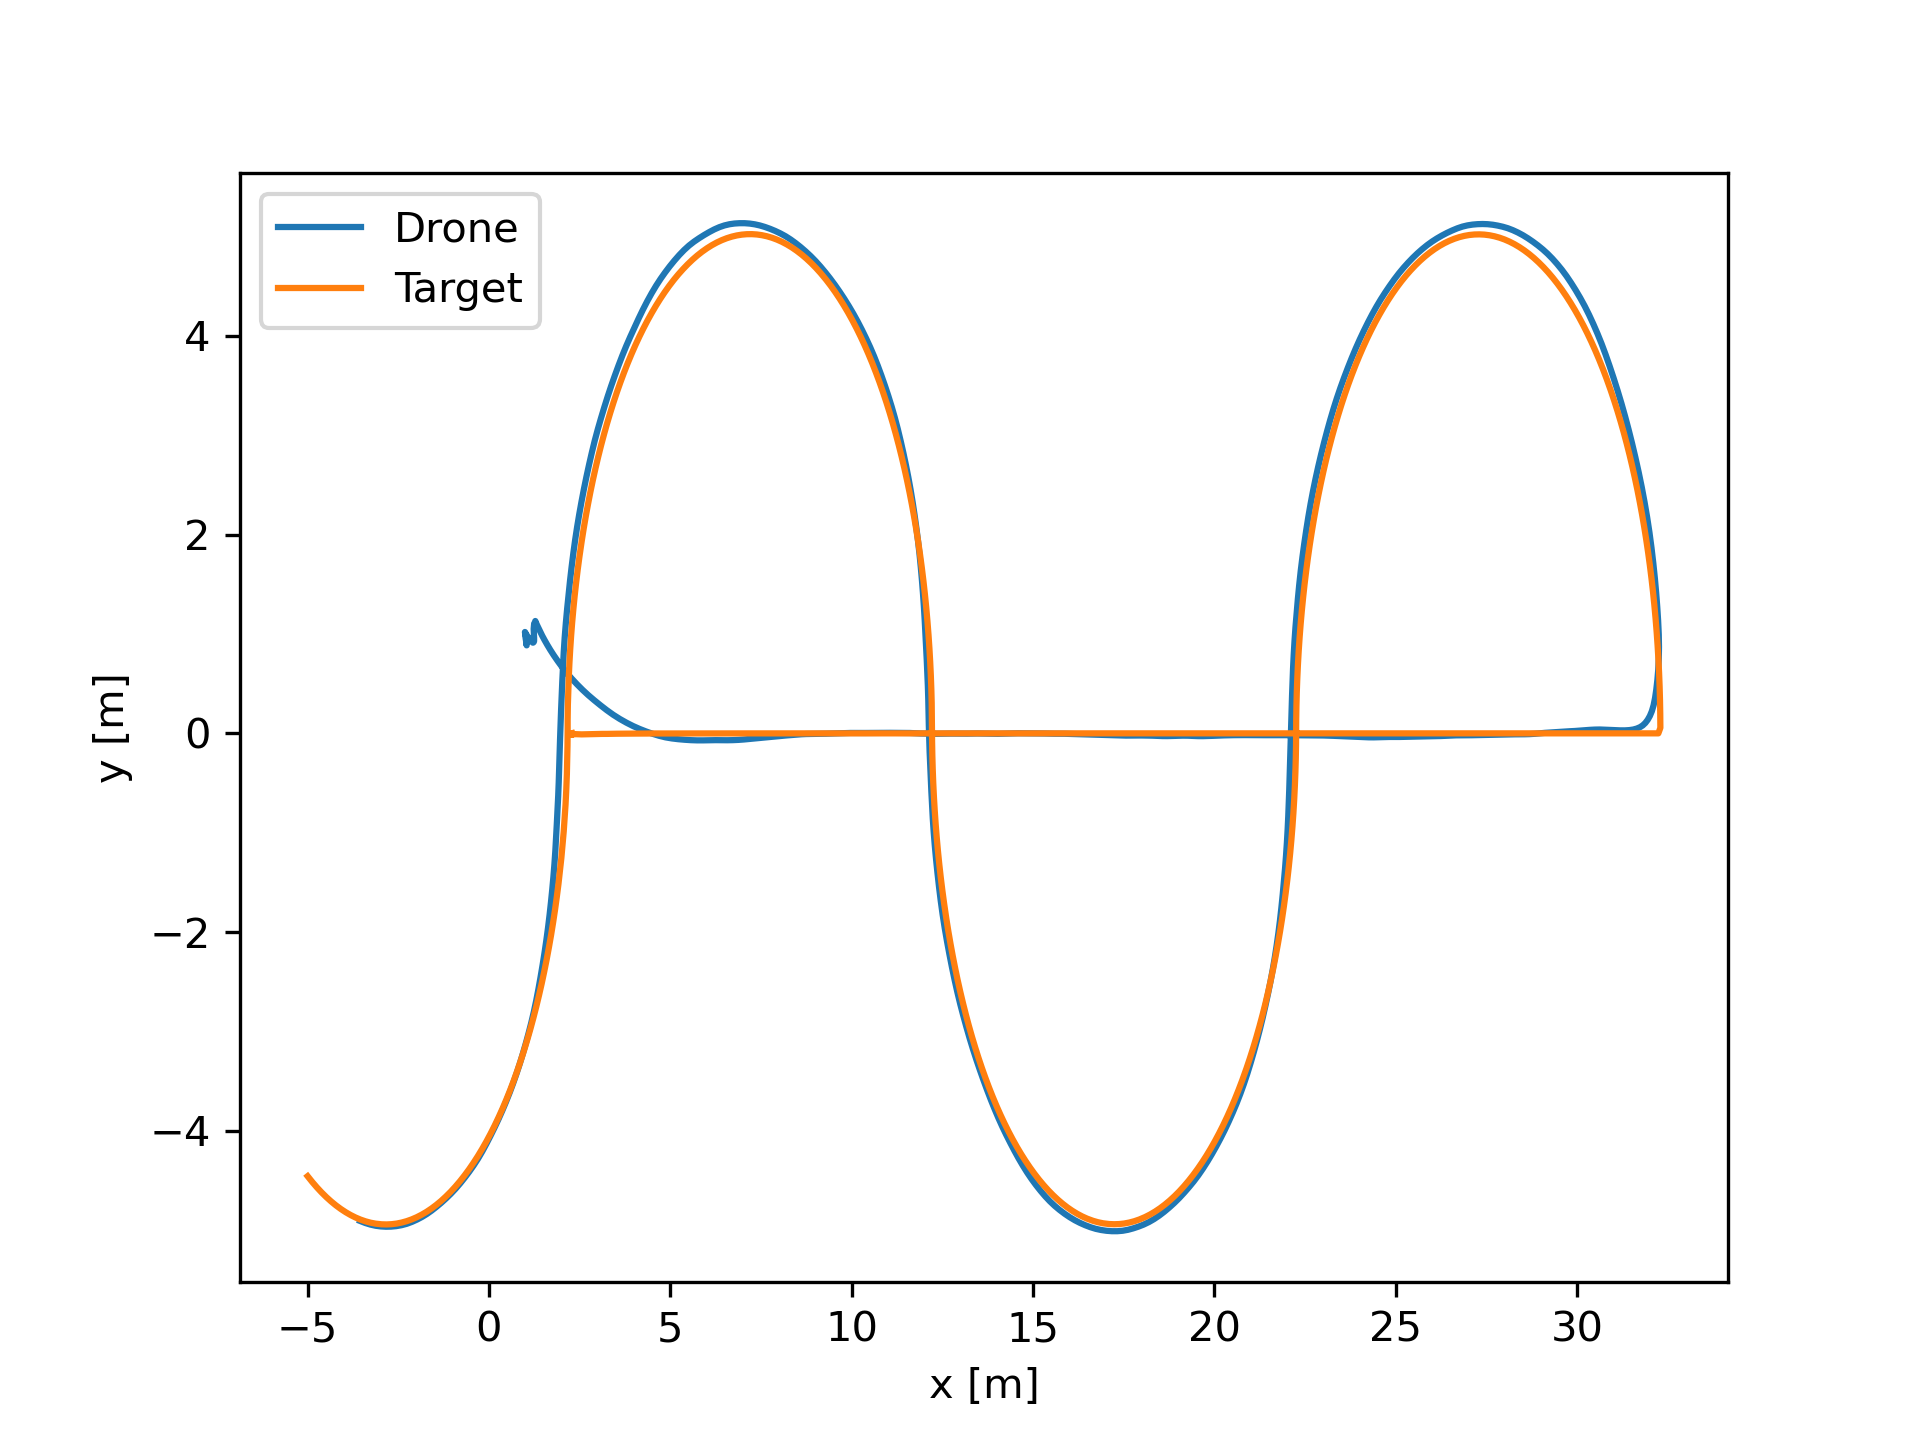
\includegraphics[width=0.48\textwidth]{images/Simulation/Drone_Target x-y Position.png}
    \caption{Target and drone trajectory in simulation.}
    \label{SIM:traj}
\end{figure}

\begin{figure}
    \centering
    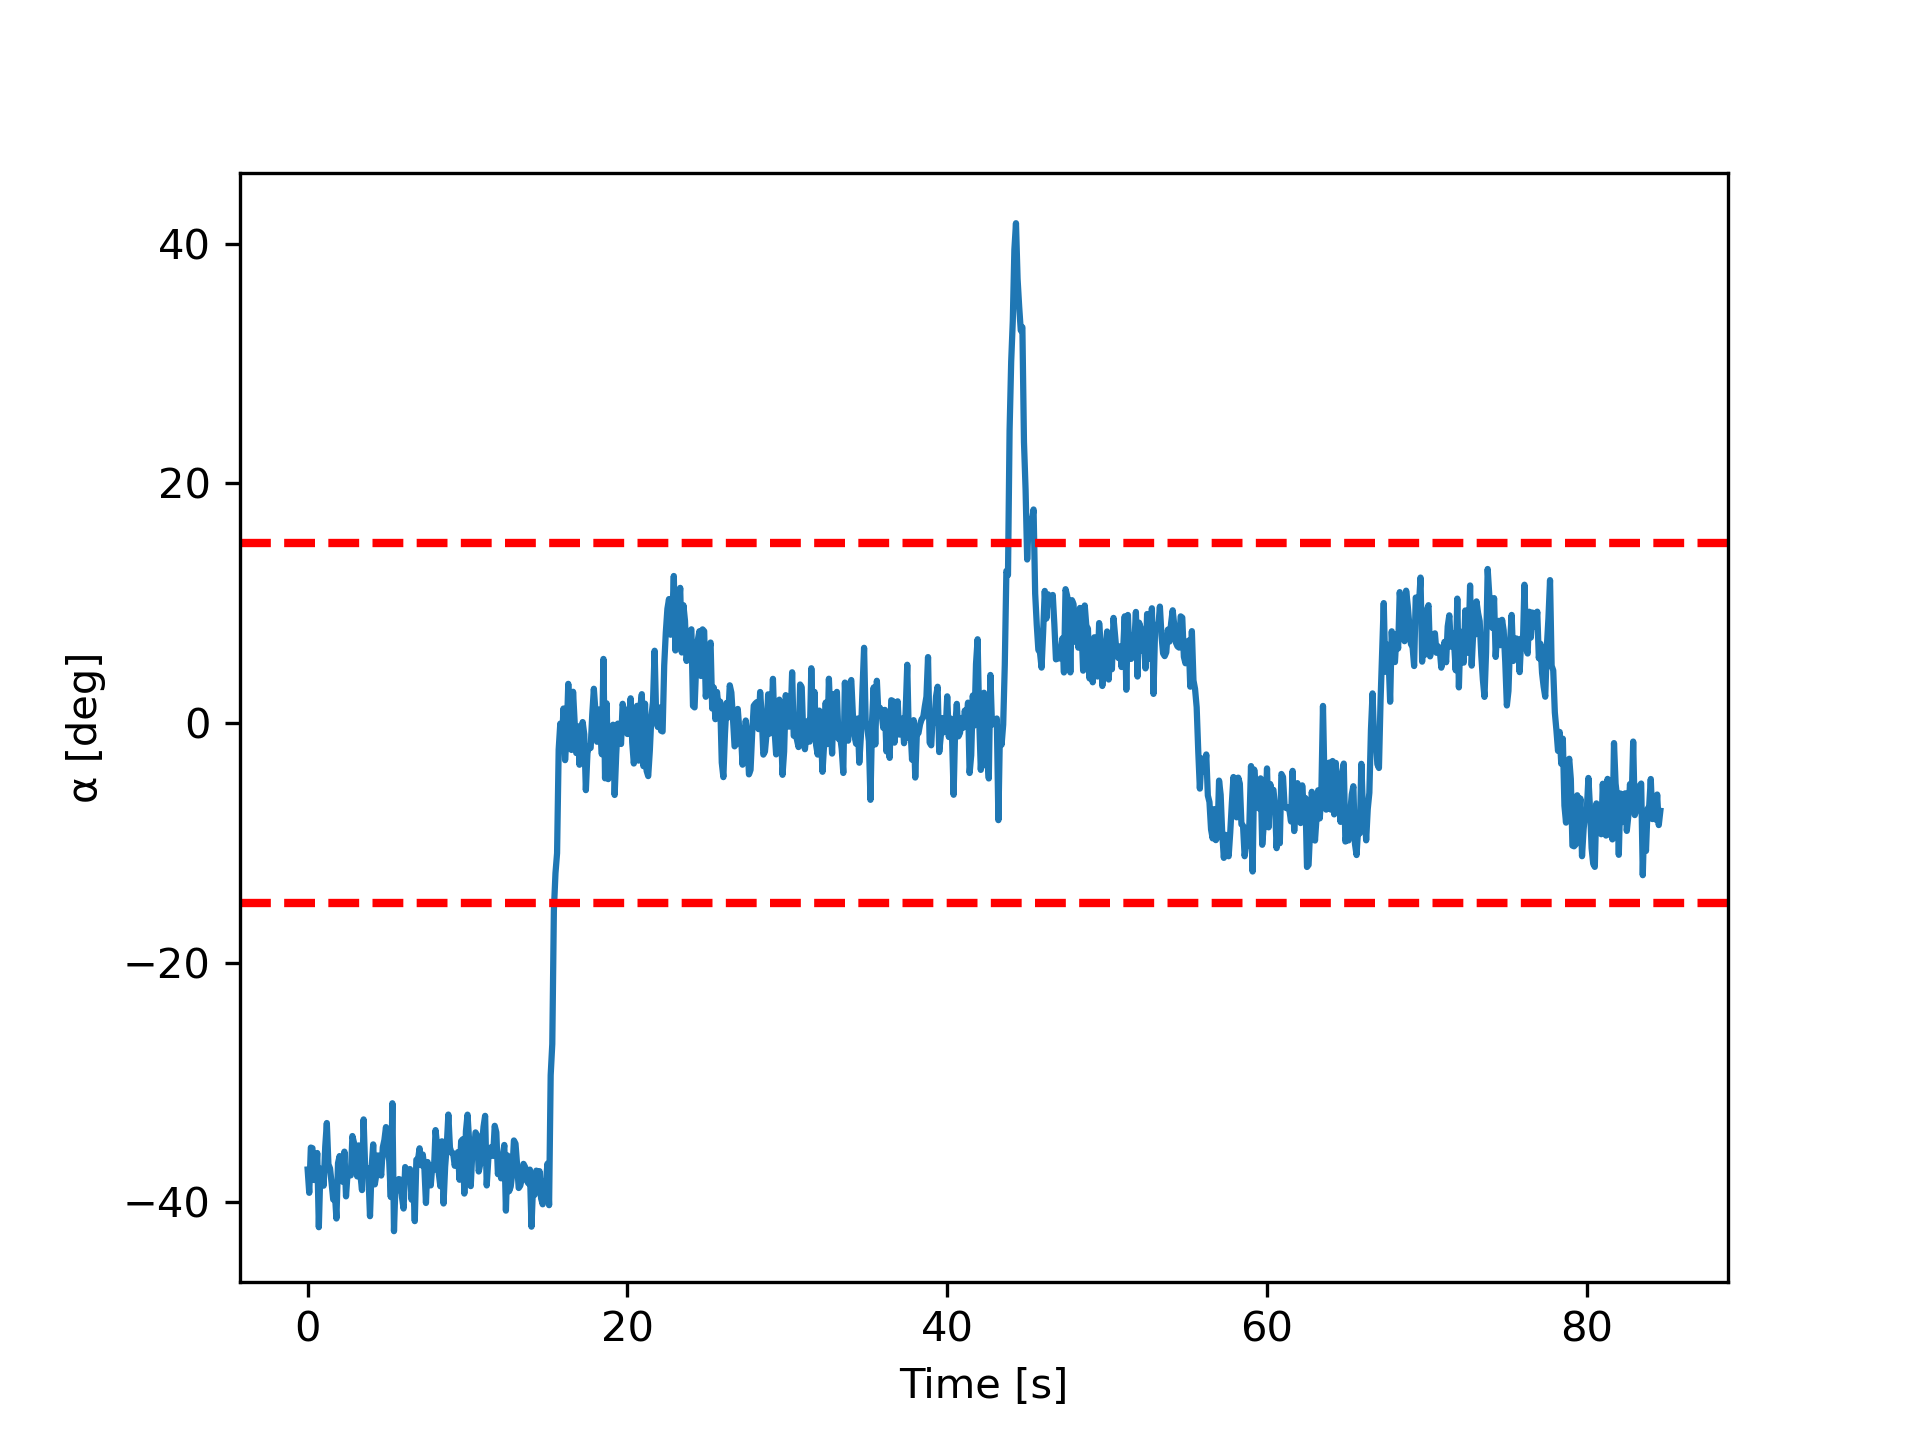
\includegraphics[width=0.48\textwidth]{images/Simulation/AoA measures.png}
    \caption{Measured AoA in simulation. The two red dotted lines, indicates the $\pm$ $15$ deg region in which the kit performs better. The fact that the measured angle remains inside this region, is an important results for the real implementation.}
    \label{SIM:aoa in time}
\end{figure}

To evaluate the performance in the following distance, \autoref{SIM:range in time} can be considered. It can be seen that on average the demanded following distance is achieved. The peak around $20$ seconds is due to the target initial movements acceleration, that instantaneously pass from a static state, to move at the set velocity. Of course the drone cannot stabilized at the same rate, so an initial gap is created. Instead the negative-positive peak pair around $40$ seconds is caused by the target's change of direction. In that moment the quadcopter stops and waits due to the presence of the integral control effect on the velocity setpoints generation, necessary to have a following distance without bias, counteracting the proportional control behaviour. Without the integral control, the proportional would cause the quadcopter to move backwards at that moment, mitigating that peak pair. However, exception made for this extreme case, our strategy seems to be appropriate so we decided to use the integral, although in some cases it may imply lowerings of the following distance. For safety purposes, in order to mitigate this effects, other strategies should be investigated.\\

\begin{figure}
    \centering
    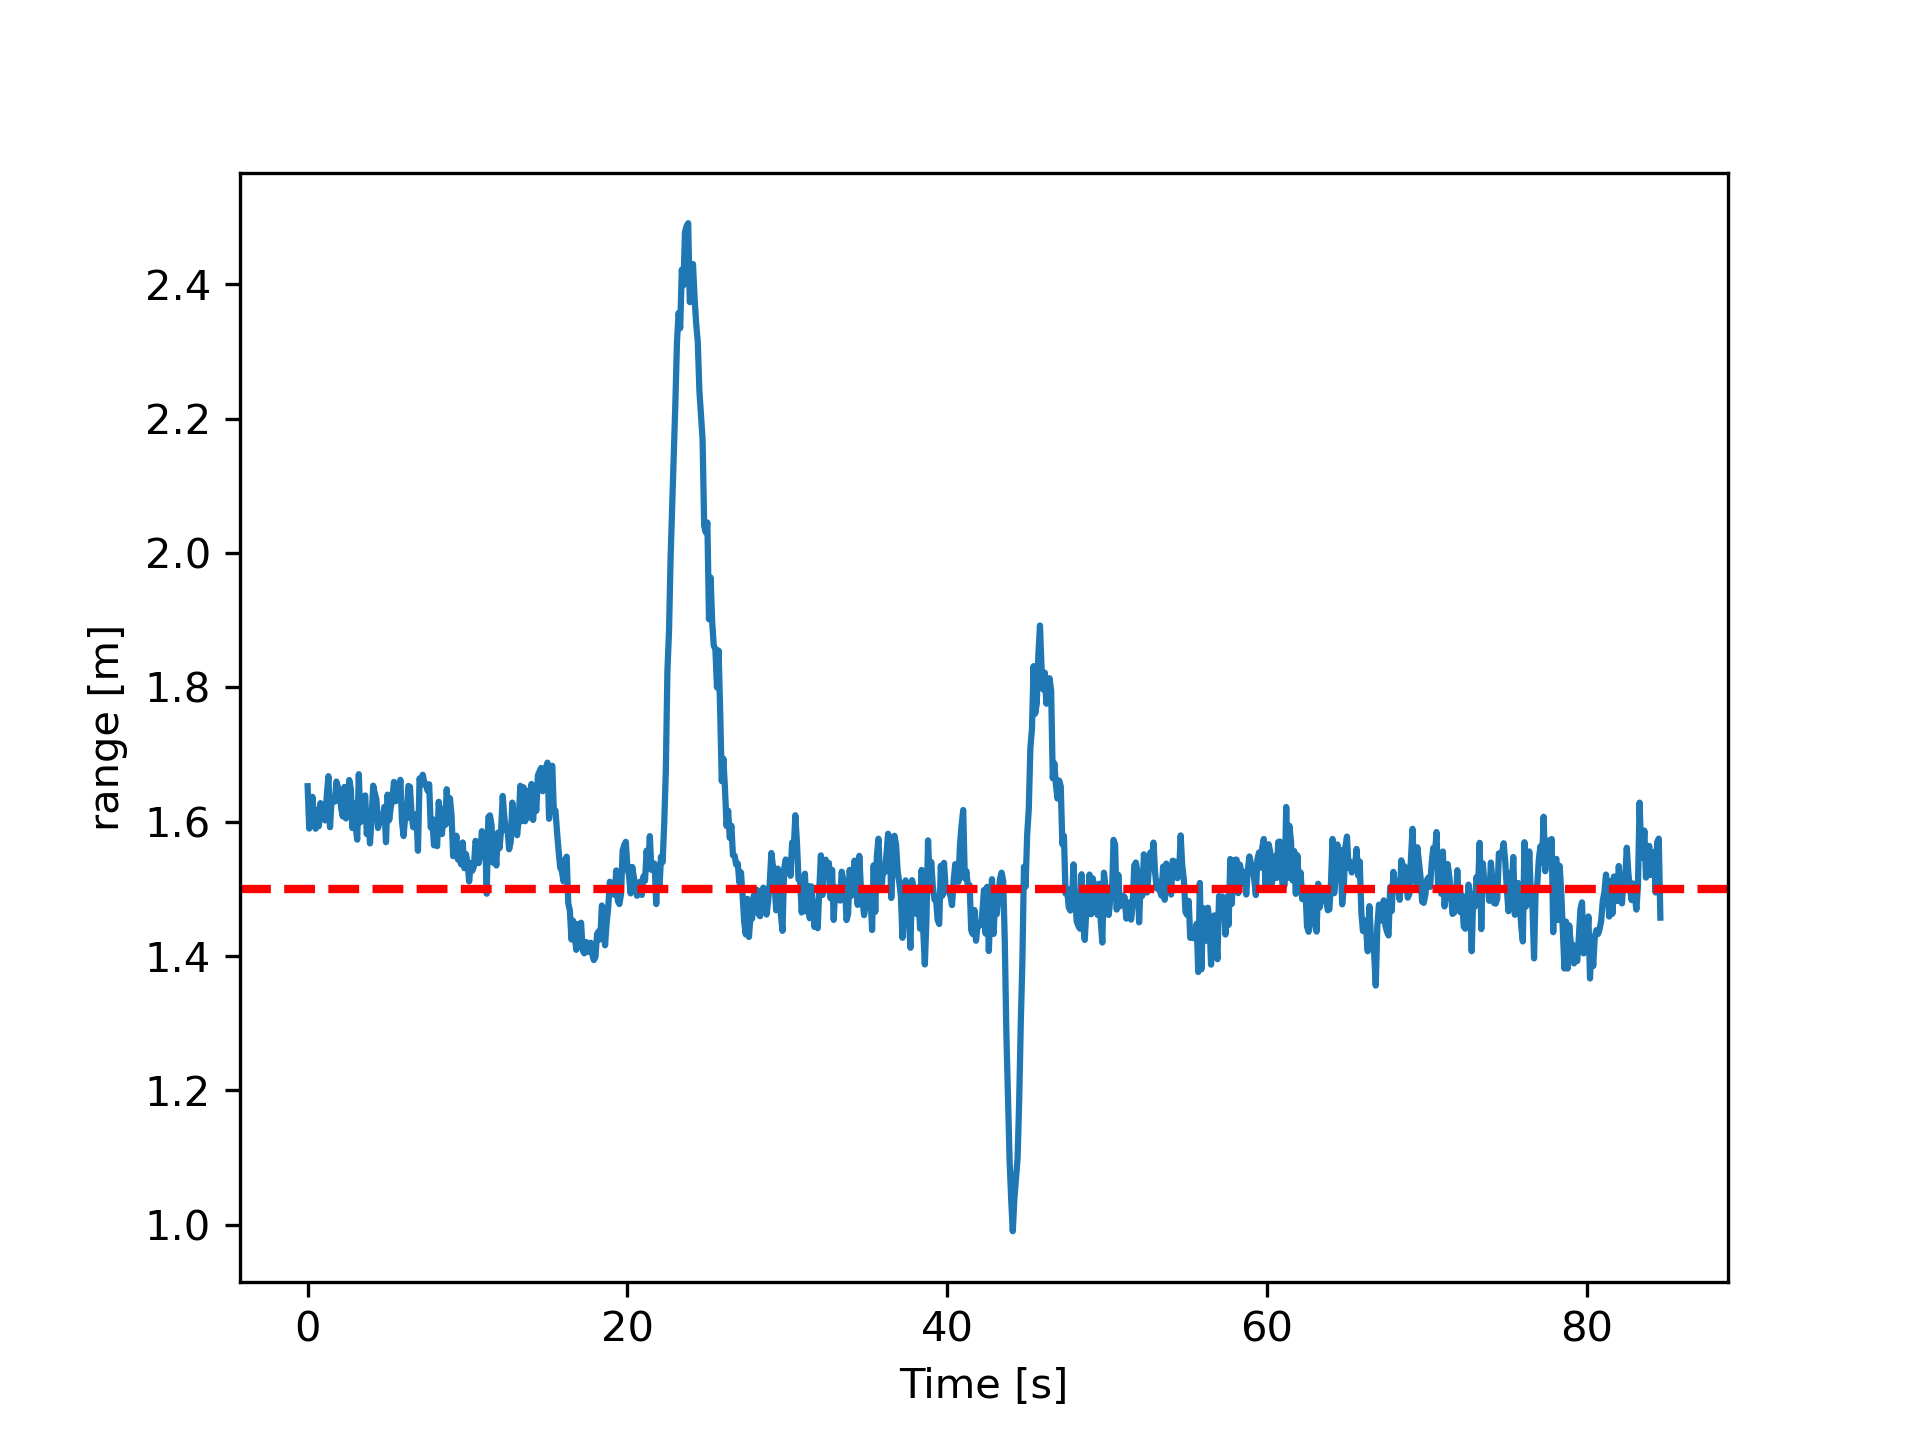
\includegraphics[width=0.48\textwidth]{images/Simulation/Range measures.png}
    \caption{Measured range in simulation. The red dotted line, indicates the wanted range from the following policy.}
    \label{SIM:range in time}
\end{figure}

\begin{figure}
    \centering
    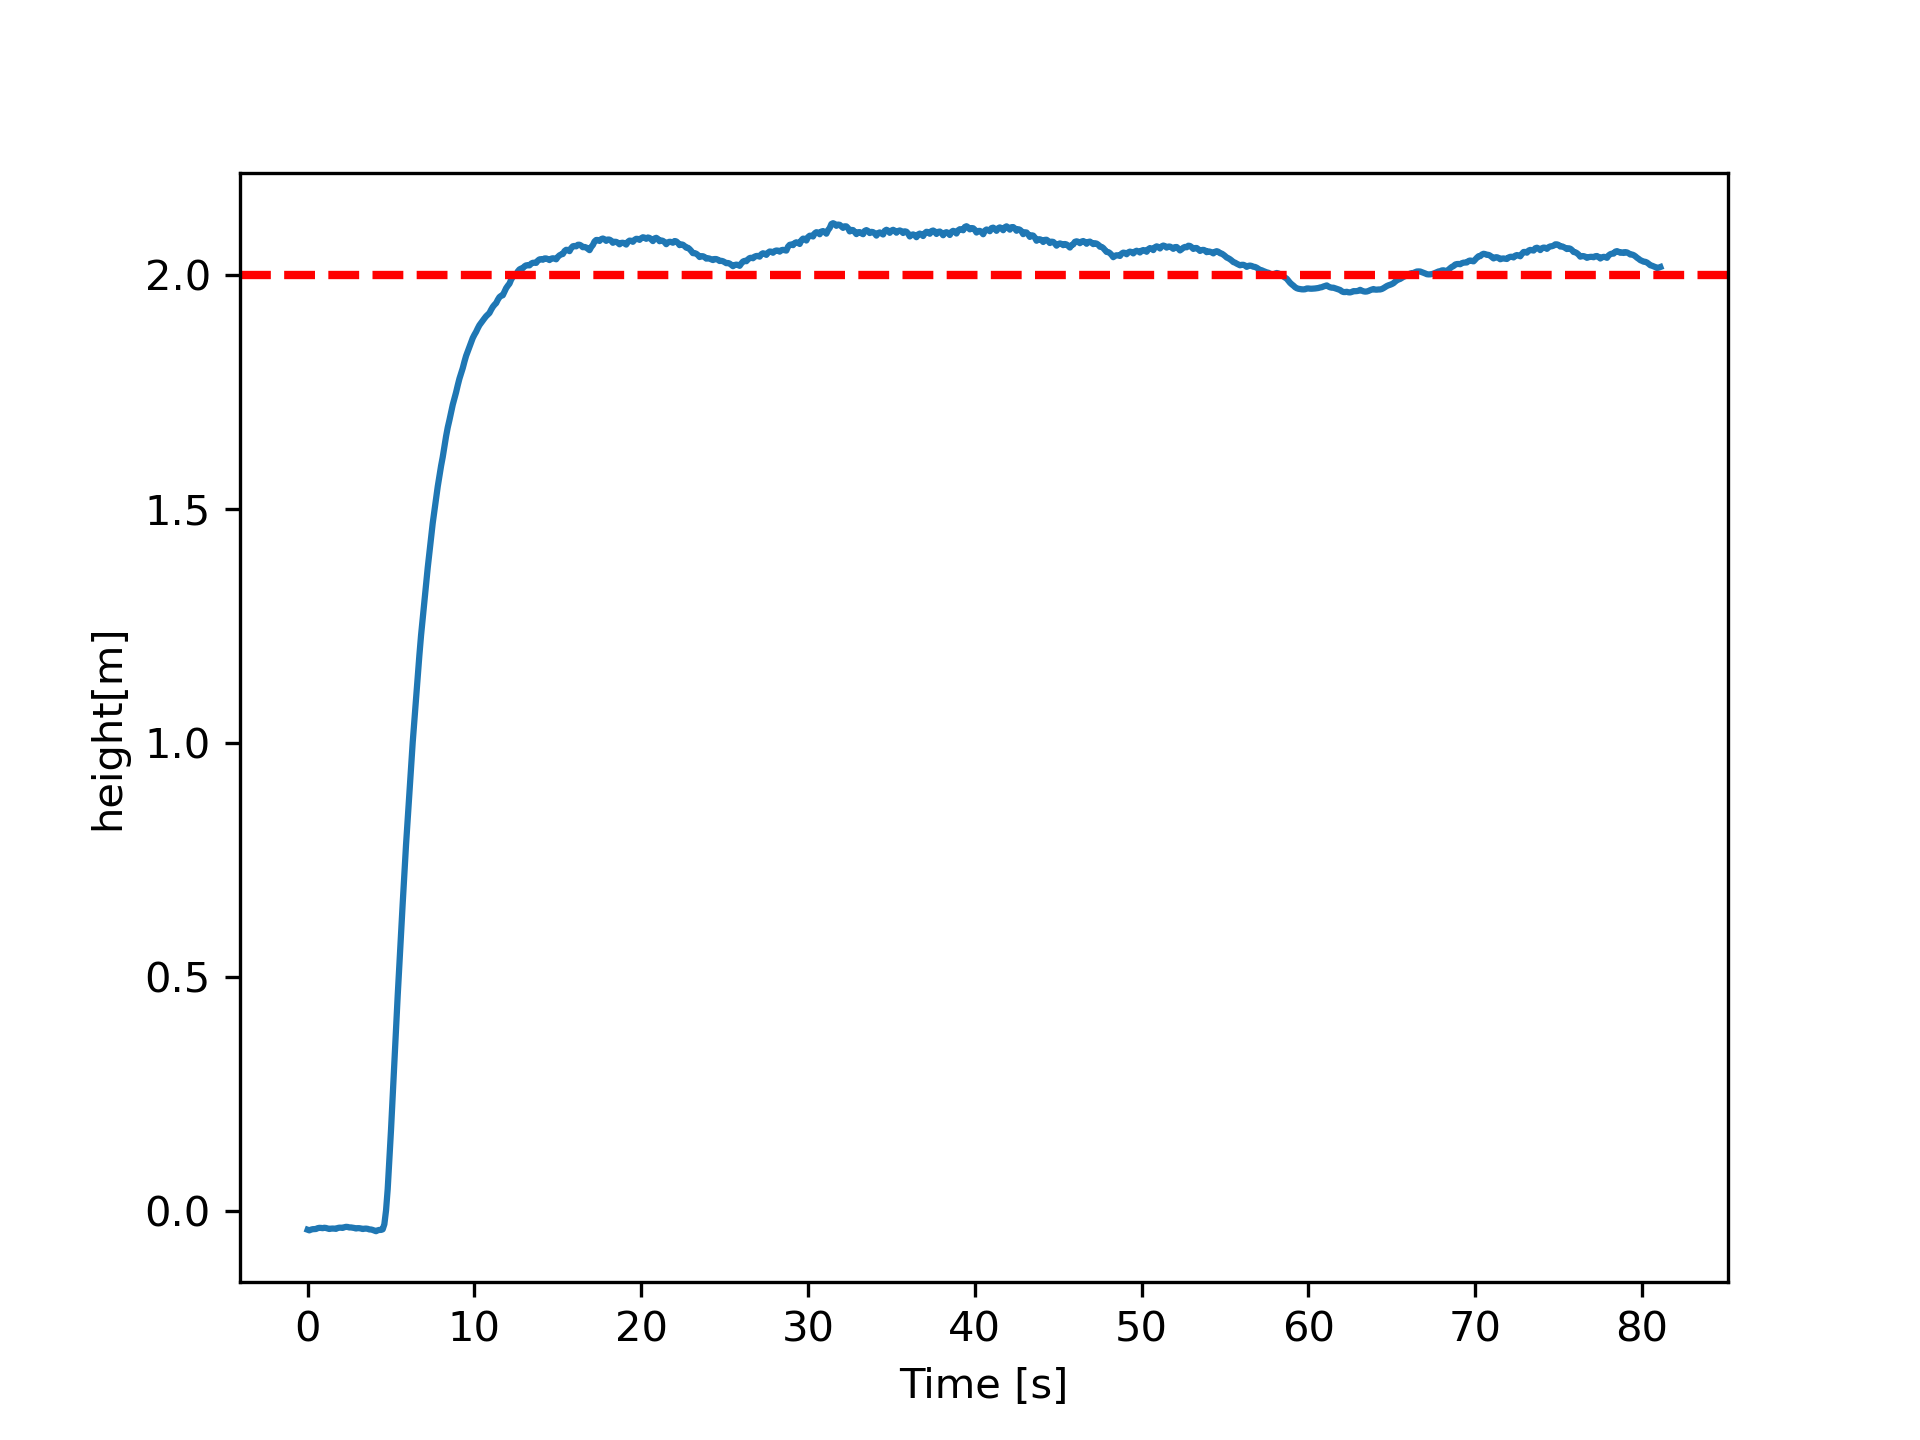
\includegraphics[width=0.48\textwidth]{images/Simulation/height_from_px4.png}
    \caption{Measured flight height in simulation. The red dotted line, indicates the wanted height from the following policy.}
    \label{SIM:height in time}
\end{figure}

Even the flight height is well respected, as can be seen in \autoref{SIM:height in time} and it seems to be independent w.r.t. events such as motion type changes. 
The estimation accuracy of the target position in the global frame done by the quadcopter using the UWB simulated sensor, is shown in \autoref{SIM:target estimation}, and it can be noted that is always reliable. More in detail, this can be seen in particular in \autoref{SIM:loc err}. The error is never greater than $0.3$ meters for both the axis. It can also be seen that is dependent on the type of motion: in the first phase, where the target move in a straight way, the error is low and approximately null on average. At the moment of the direction change, when the target starts the curved motion, it expands for both the axis and the mean done on a window relative to that moment is not null. However, the fact that the error is never too large guarantees acceptable following performance.\\

\begin{figure}
    \centering
    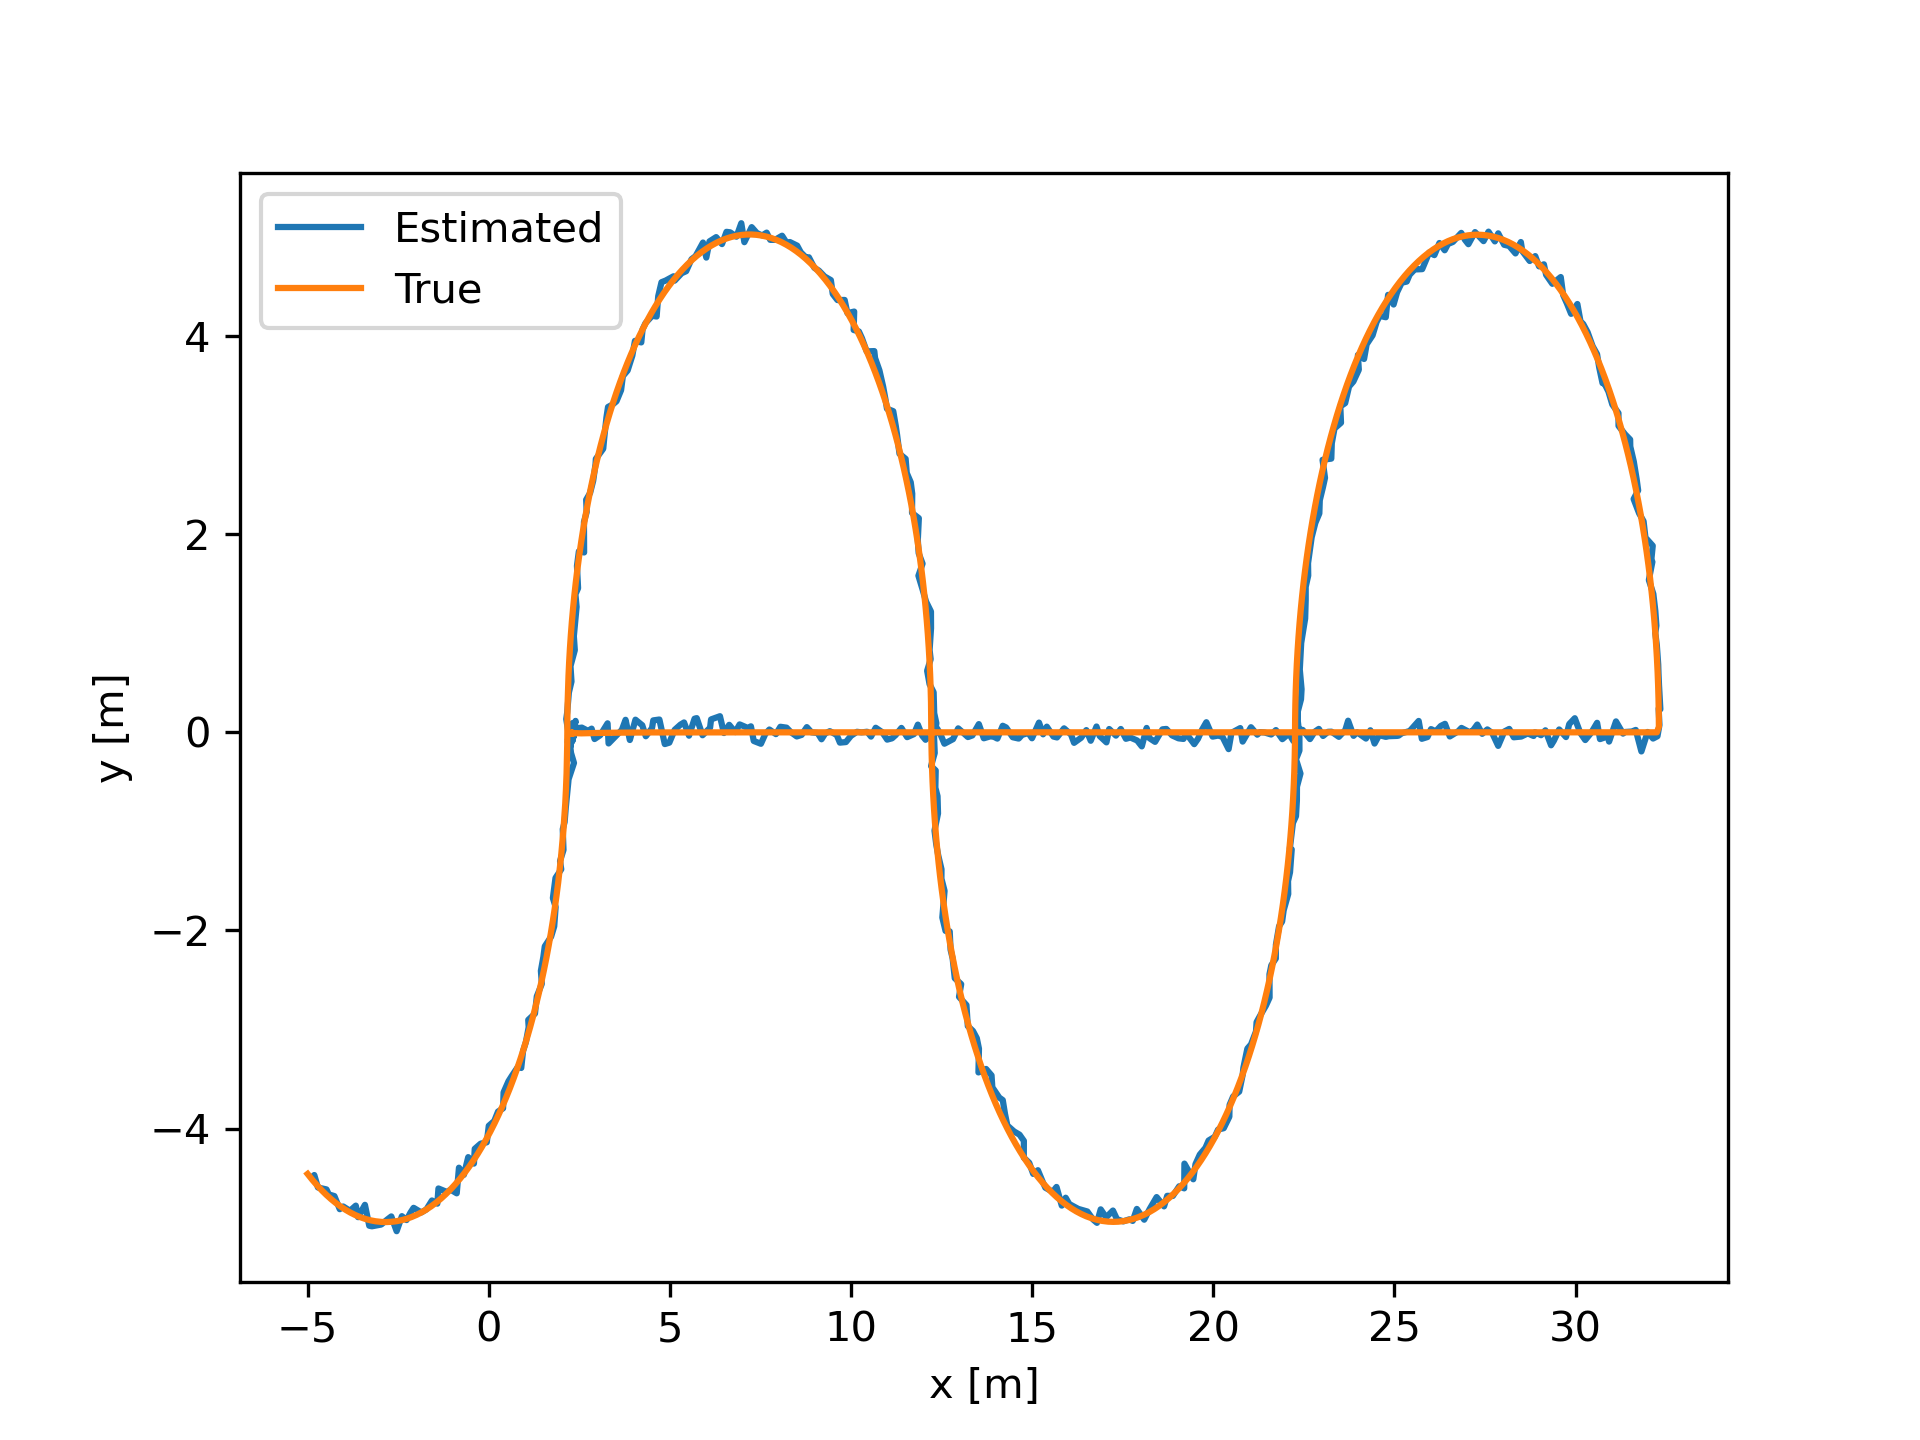
\includegraphics[width=0.48\textwidth]{images/Simulation/tag_estimation_vs_real.png}
    \caption{True and estimated pose of the target.}
    \label{SIM:target estimation}
\end{figure}

\begin{figure}
     \centering     
     \subfigure[]{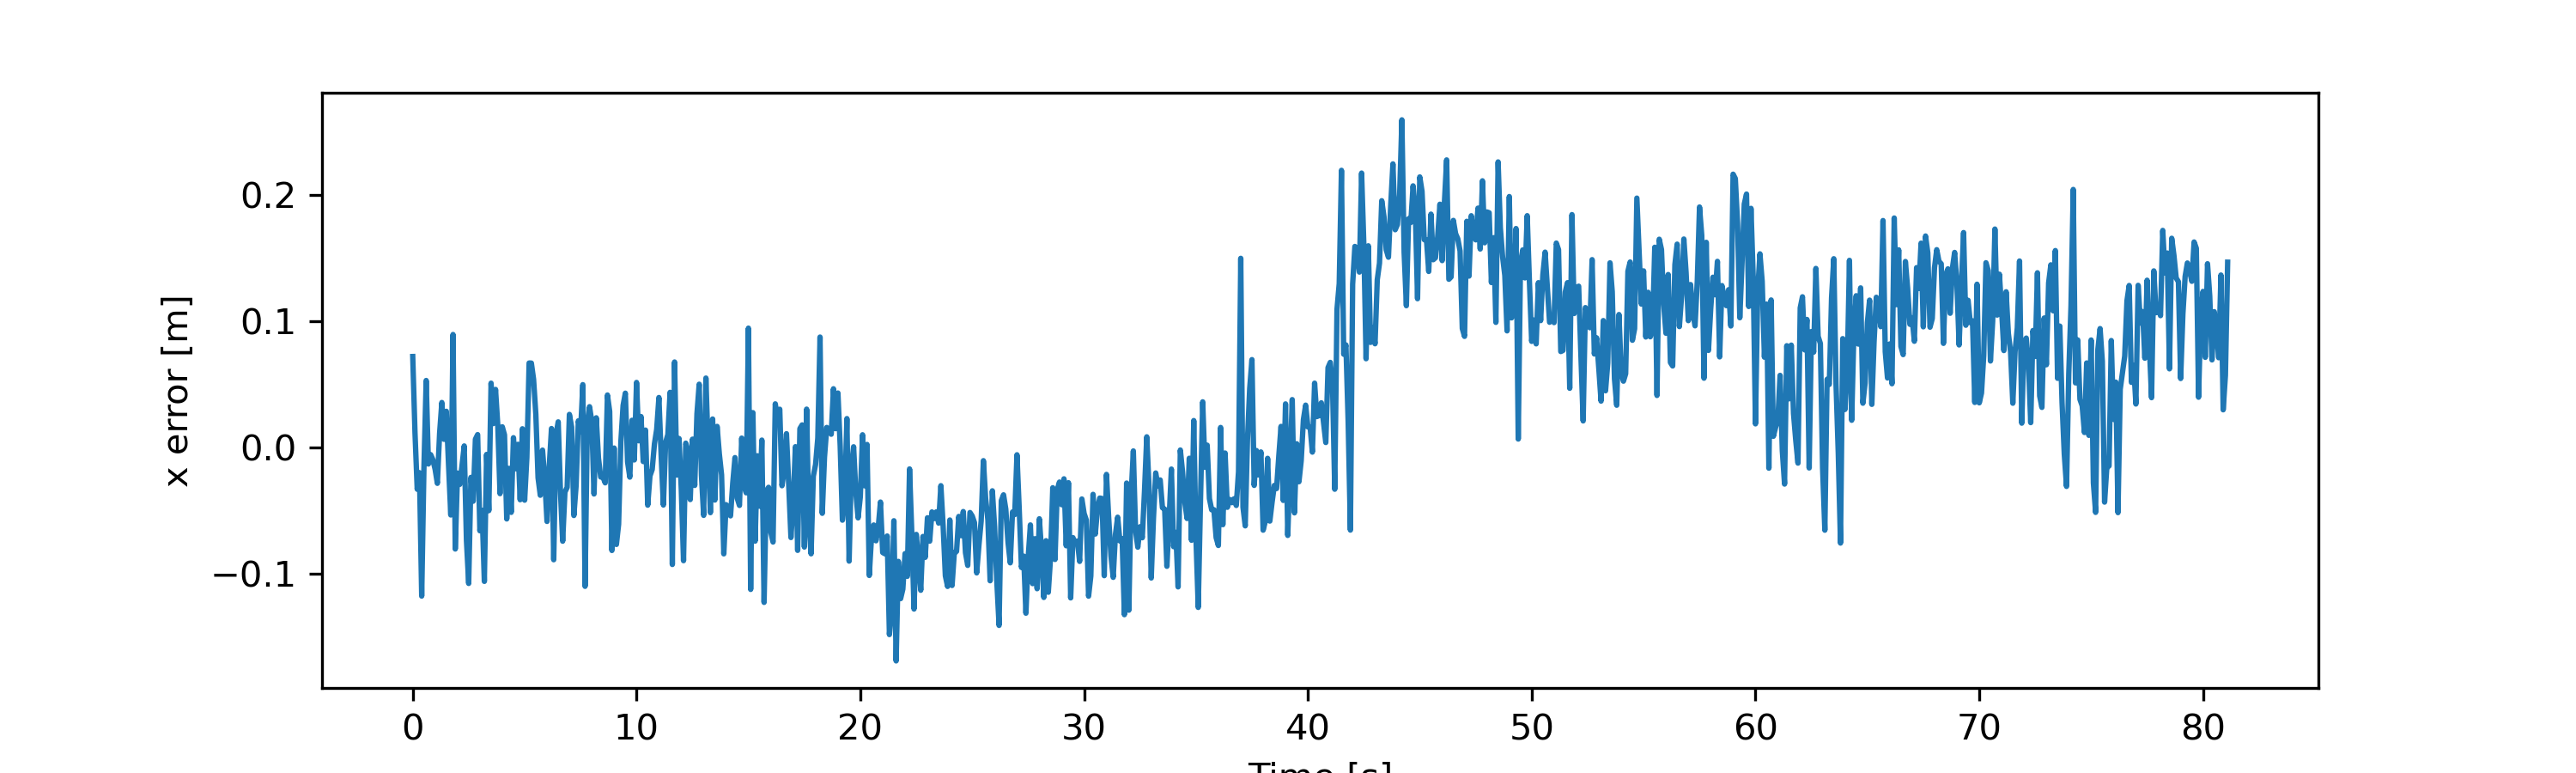
\includegraphics[width=0.48\textwidth]{images/Simulation/tag_estimation_errx.png}}\\
     \subfigure[]{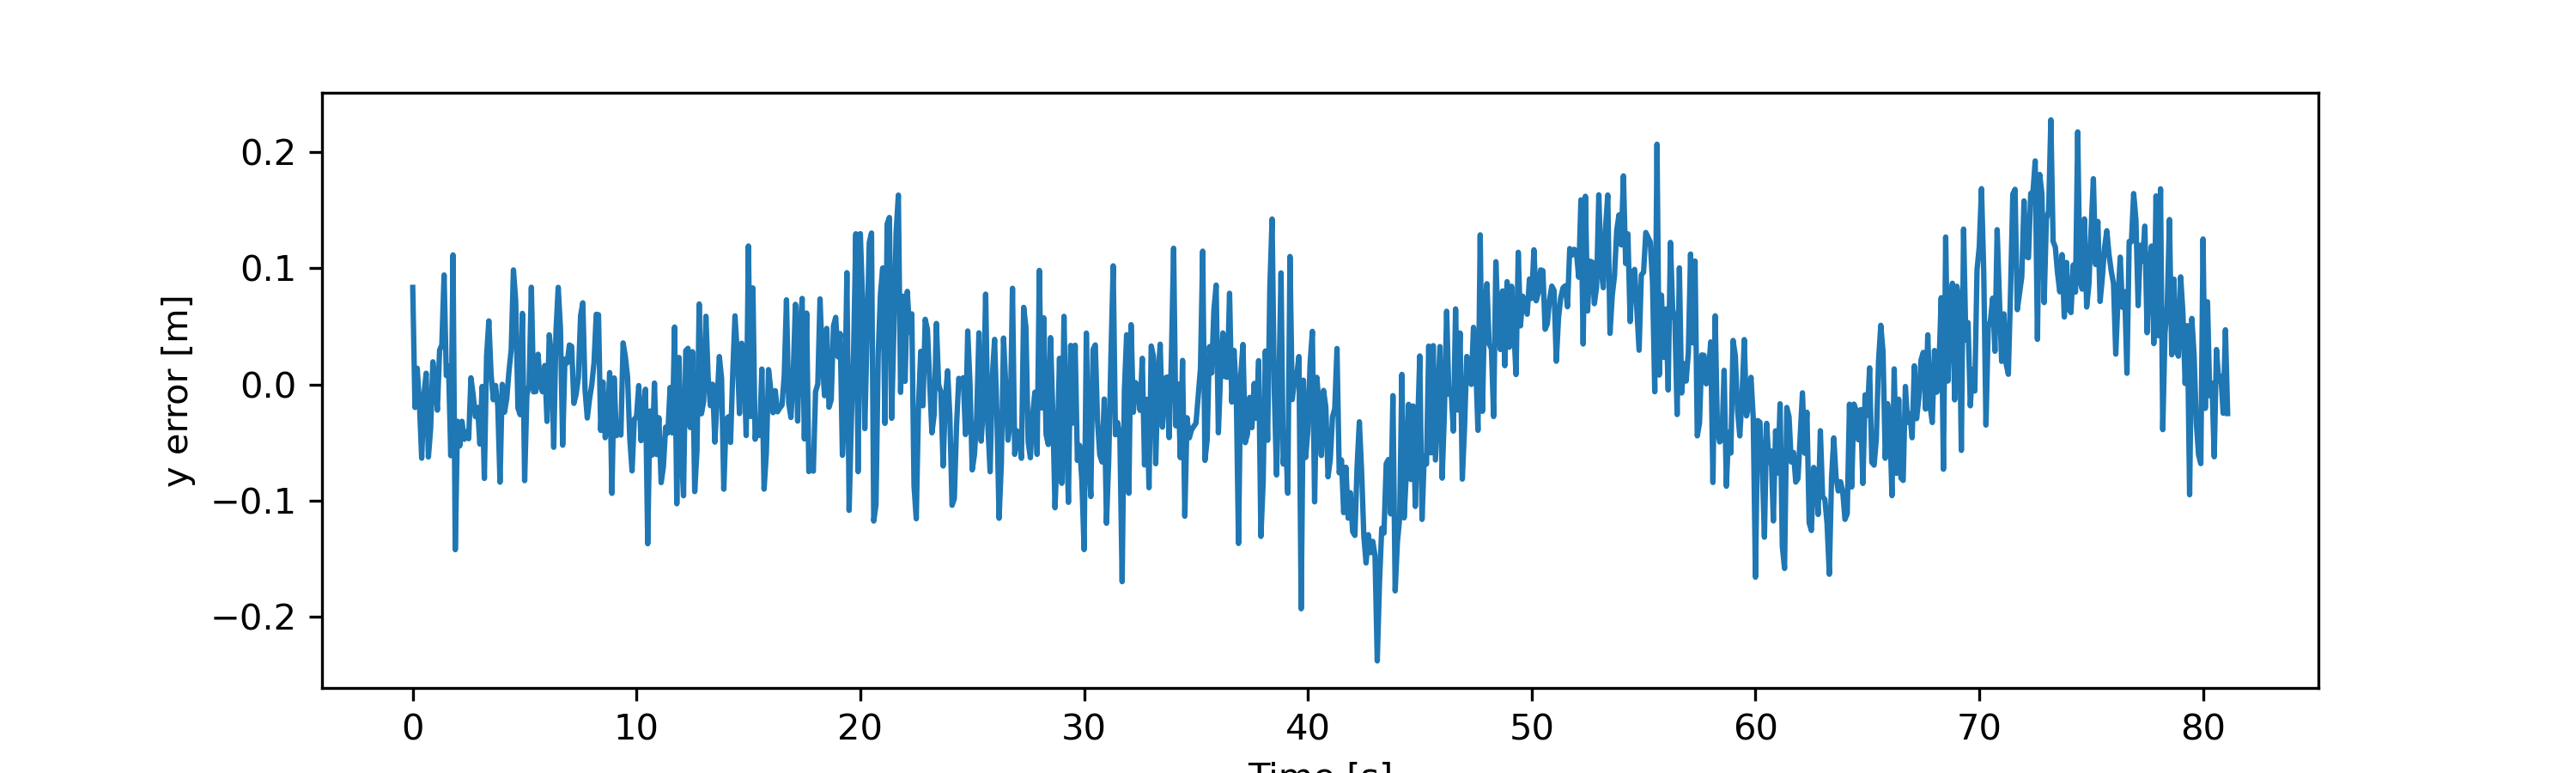
\includegraphics[width=0.48\textwidth]{images/Simulation/tag_estimation_erry.png}}
     \caption{(a) target localization x error [m]. (b) target localization y error [m].}
     \label{SIM:loc err}
\end{figure}

To test the robustness of the following system, a simulation with noises affected by larger standard deviations, $10$ centimeters for the range and $10$ degrees for the AoA was performed. From \autoref{SIM:traj_noisy}, it can be seen that the quadcopter is still able to execute its task, albeit roughly.\\
Overall, these results suggests that our strategy works, at least in the simulated conditions: some effects indeed are neglected, as the fact that the quadcopter used in the real application, is smaller and different from the simulated Iris drone as well as the inertial modifications due to the mounted UWB sensor, that are not considered. 

\subsection{Real test}
To test the validity of the UWB kit in a real application, and to further prove the effectiveness of the following algorithm, as previously explained, some real tests where performed. All the presented results are paired with the relative MoCap ground truth for comparison. The presented results are the best of the conducted tests. In order to obtain a decent motion inside the restricted Mocap laboratory environment, the test were conducted choosing a drone flight height of $0.4$ meters (to ensure marker visibility) and a following distance of $1.2$ meters. This choice is for sure restricting the UWB kit performance, since better results are obtained at larger distances (as suggested by the manufacturer), but this choice is restricted by the lab dimensions that do not allow to perform good trajectories with higher distances.\\

In \autoref{REAL:fig:traj} the trajectory of both drone and target, given by MoCap, are presented. It is clear that the drone almost follow the square-like trajectory of the target, suggesting the effectiveness of the following strategy. For what concerns the policy compliance, in \autoref{REAL:fig:aoa}, \ref{REAL:fig:range} AoA and range obtained by the sensor with the relative MoCap ground truth, are depicted. From both can be highlighted the presence of a non-linear bias that majorly depends by the angle. This confirms the behaviour seen in the characterization, in which the angle bias is a function of the actual angle. Nonetheless, the error is maximum in the target turning phases, in which the DDR robot makes almost sharp change of direction. This concretize the behavior mentioned in the characterization conclusions, for which the measures are worsen by a non radial facing of the tag w.r.t. the double UWB. All these effects sum up, obtaining a non constant bias, especially for the AoA. Nevertheless, if we do not consider the biases, in general the policy is followed. Surely, an outdoor test performed in an open environment, with a more relaxed policy (i.e. a greater following distance), should achieve better results. For what concerns the height, as described, is controlled directly by sending constants z setpoints. The flight height followed by the quadcopter, is presented in \autoref{REAL:fig:height}. The height is maintained with an error similar to the one of the simulation.\\

\begin{figure}
    \centering
    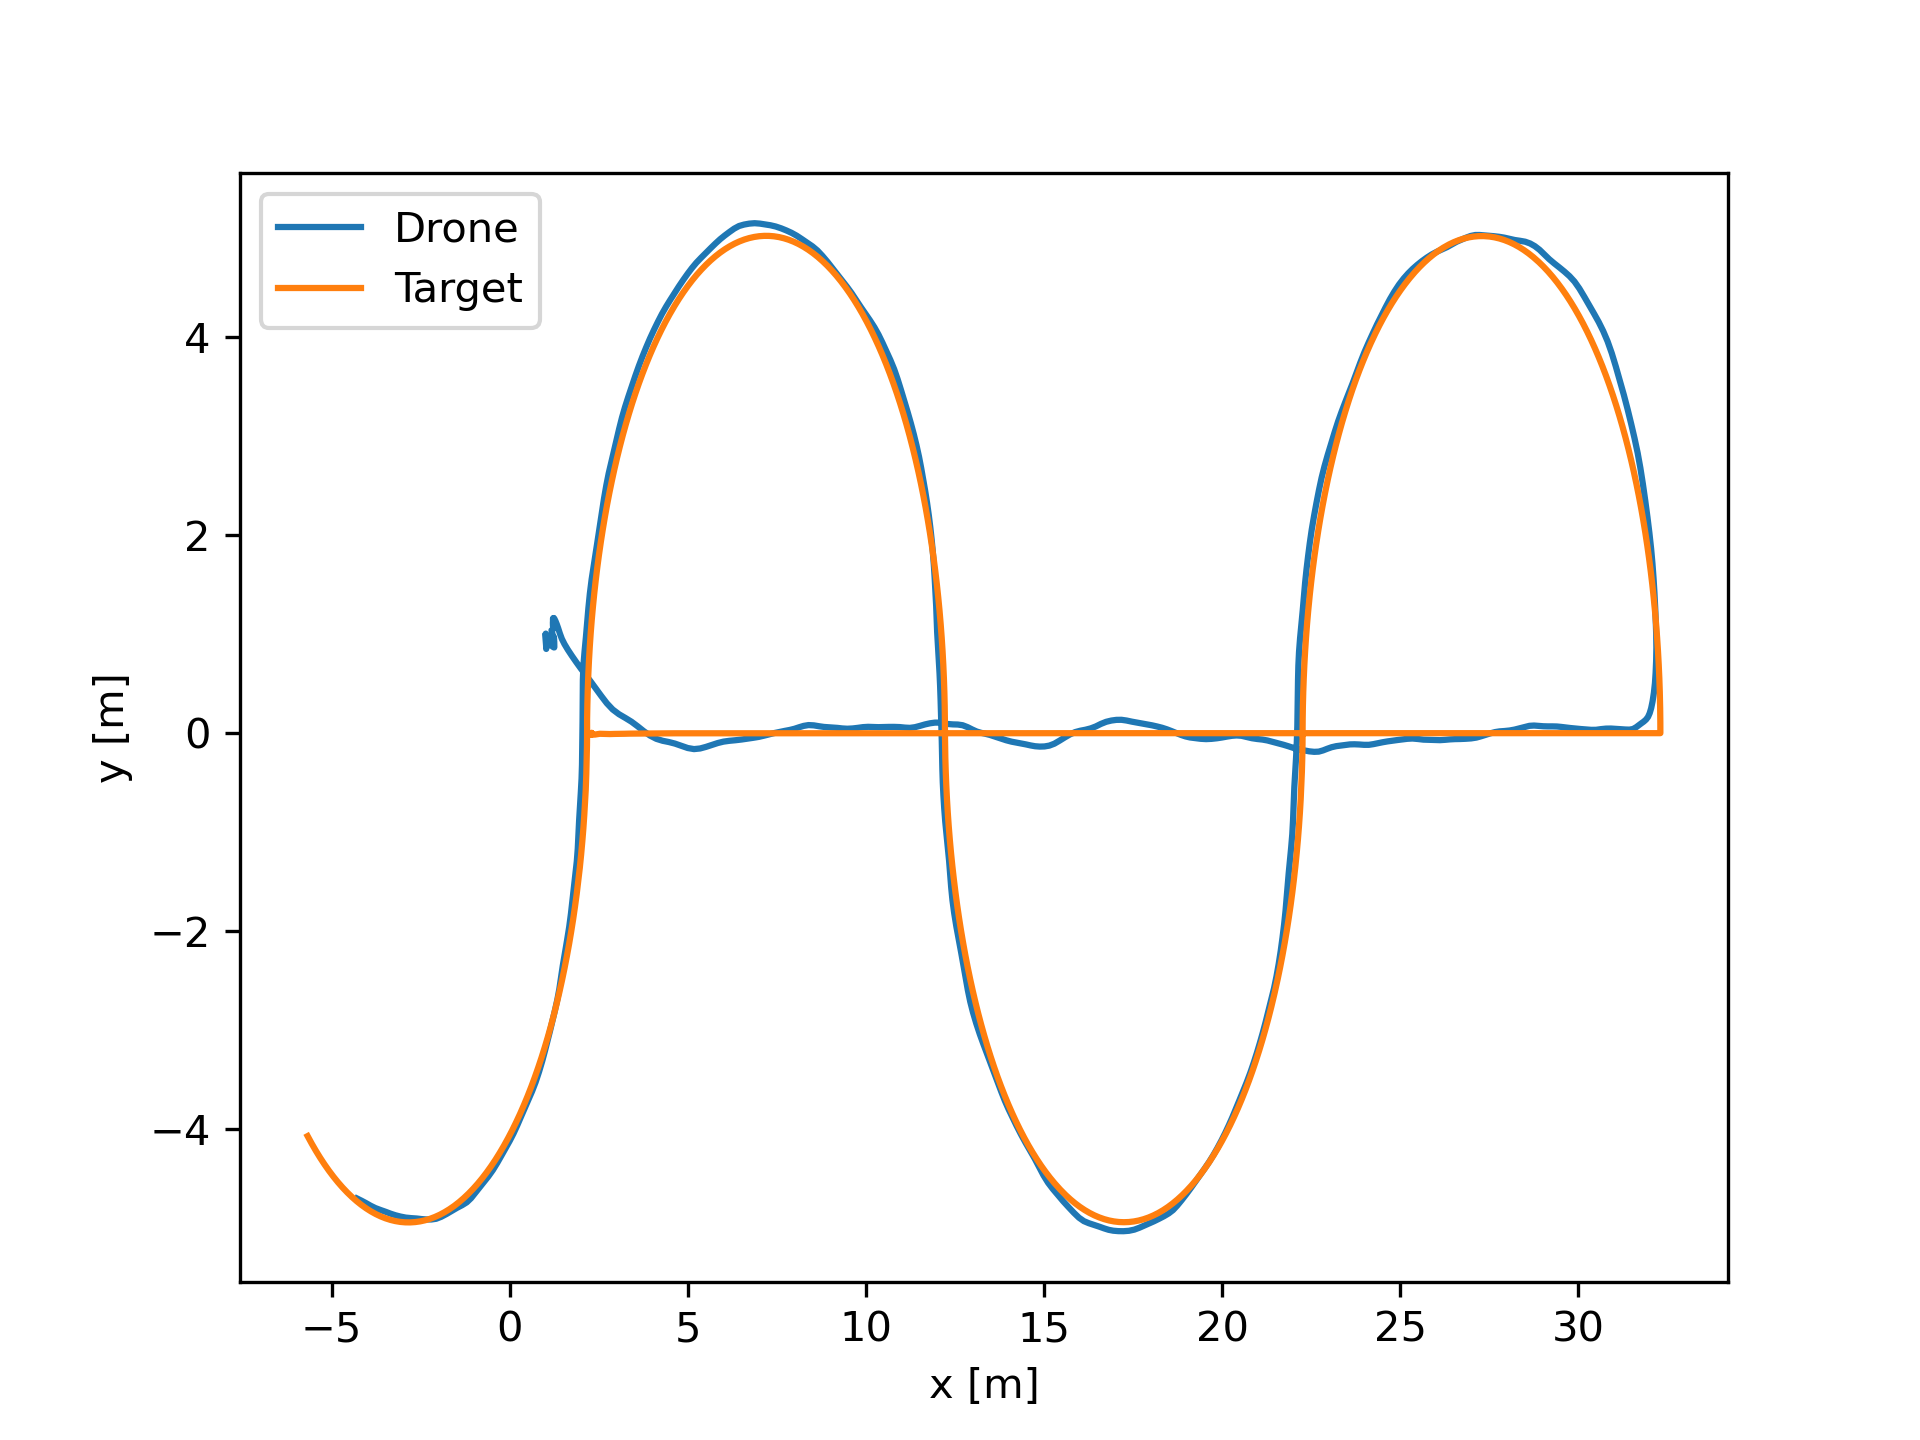
\includegraphics[width=0.48\textwidth]{images/Simulation/Drone_Target x-y Position_noisy.png}
    \caption{Target and drone trajectory in simulation with high noise.}
    \label{SIM:traj_noisy}
\end{figure}

\begin{figure}
    \centering
    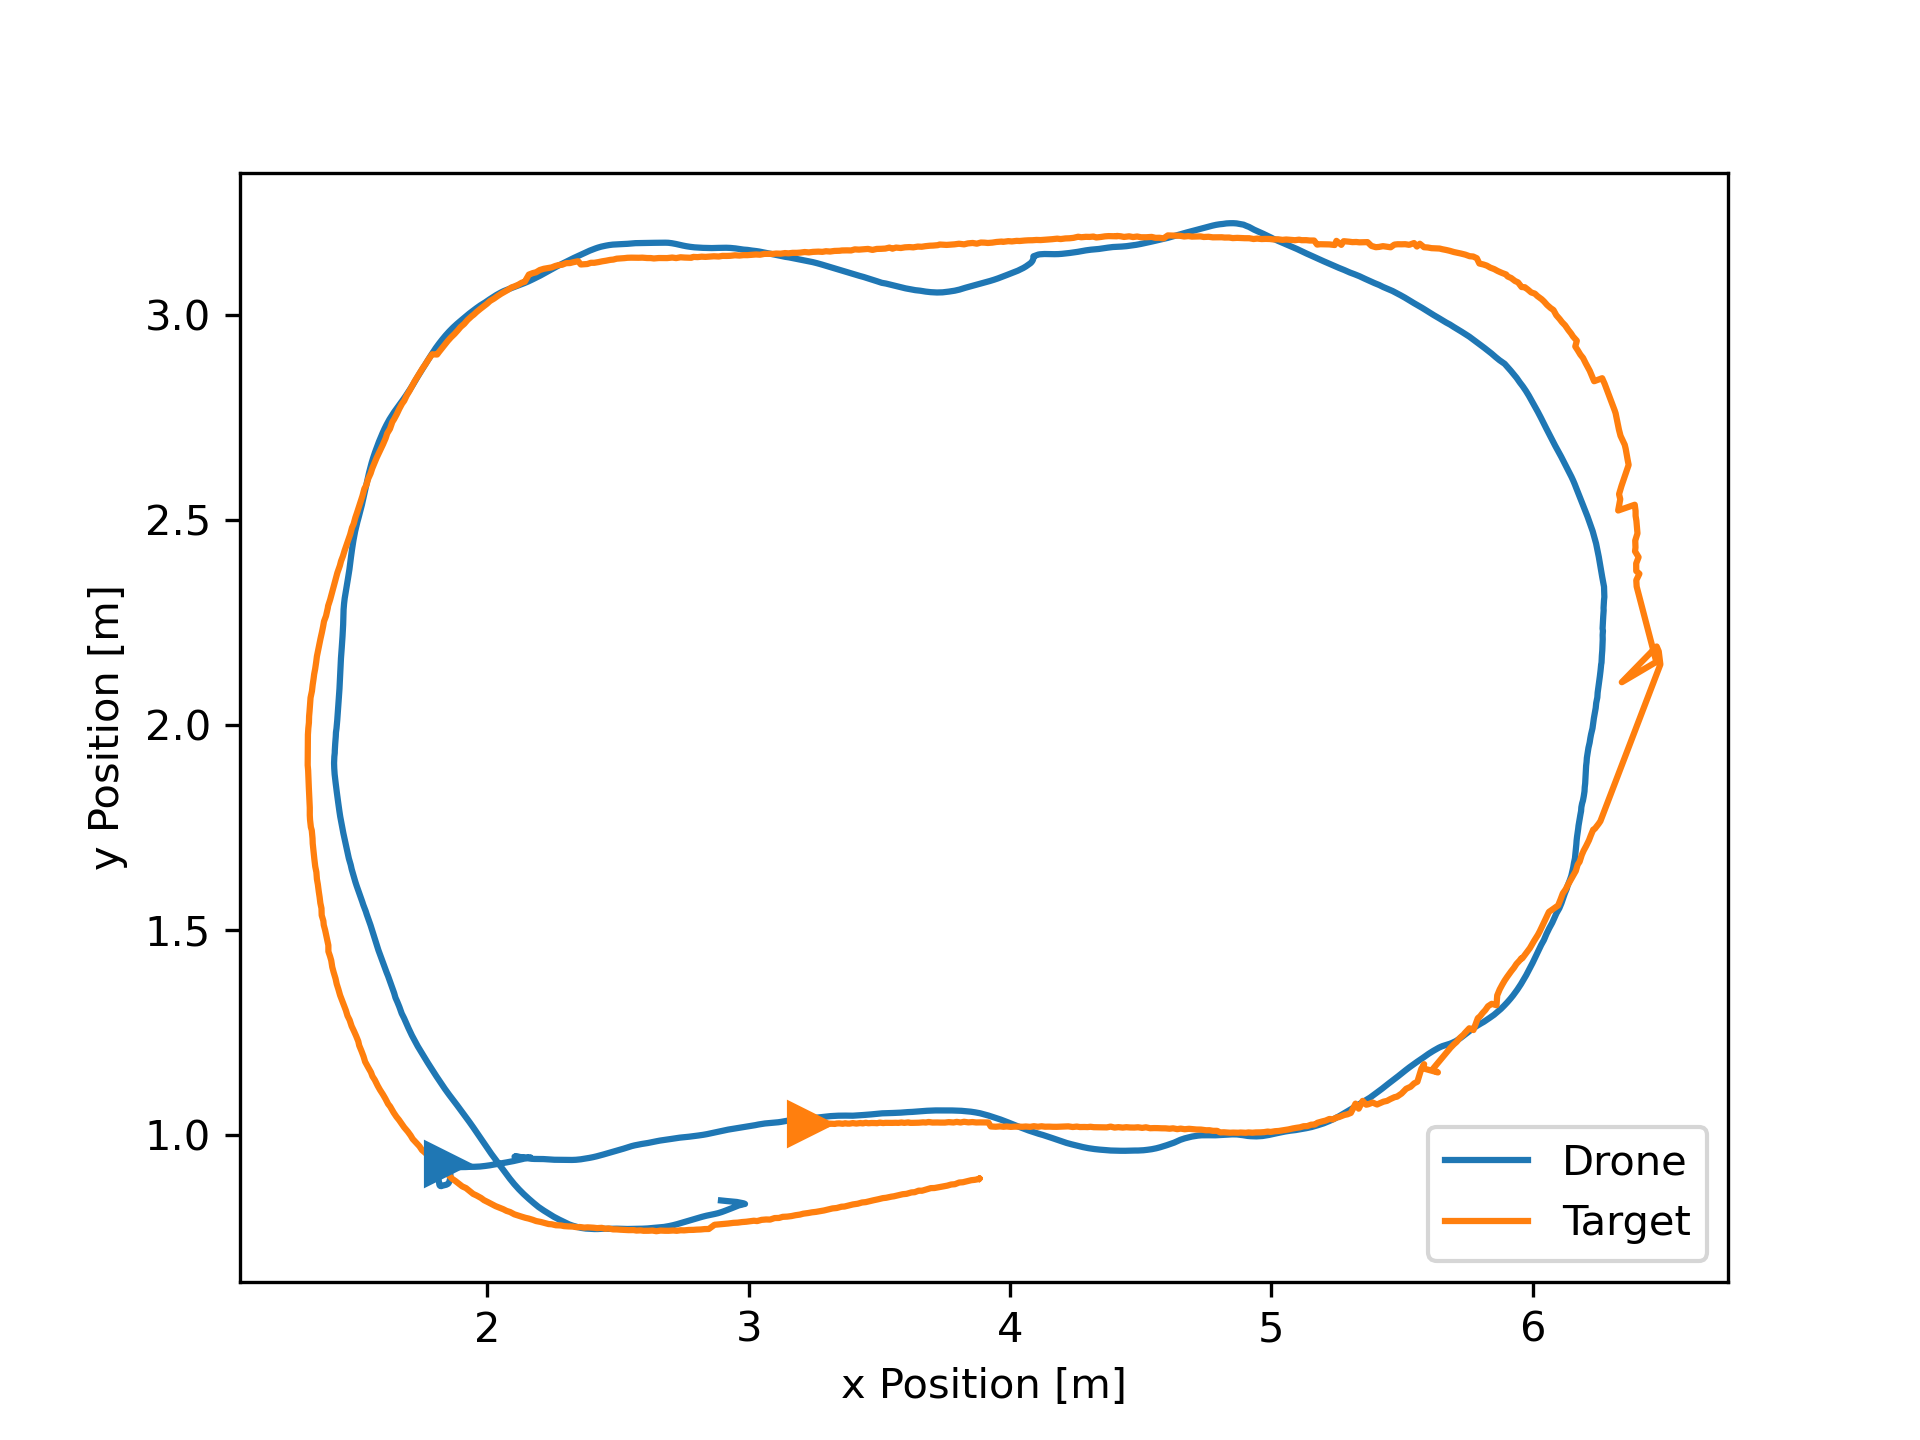
\includegraphics[width=0.48\textwidth]{images/real_test/drone_target_xy_pos.png}
    \caption{Target and drone trajectory in real test.}
    \label{REAL:fig:traj}
\end{figure}

The accuracy of the target position drone's estimate, performed using the UWB sensor and its own position estimate, is shown in \autoref{REAL:fig:tag_estim}. As can be seen, the estimate follows in general the truth, but is clearly affected by the angle and range biases previously discussed. To better asses the localization performance, the x and y error in time are exposed in \autoref{REAL:fig:loc_err}. The error in both the axes, is bounded in $\pm 0.4$ meters, which is almost twice the one obtained in the simulation. This is clearly due to the described biases.\\

\begin{figure}
    \centering
    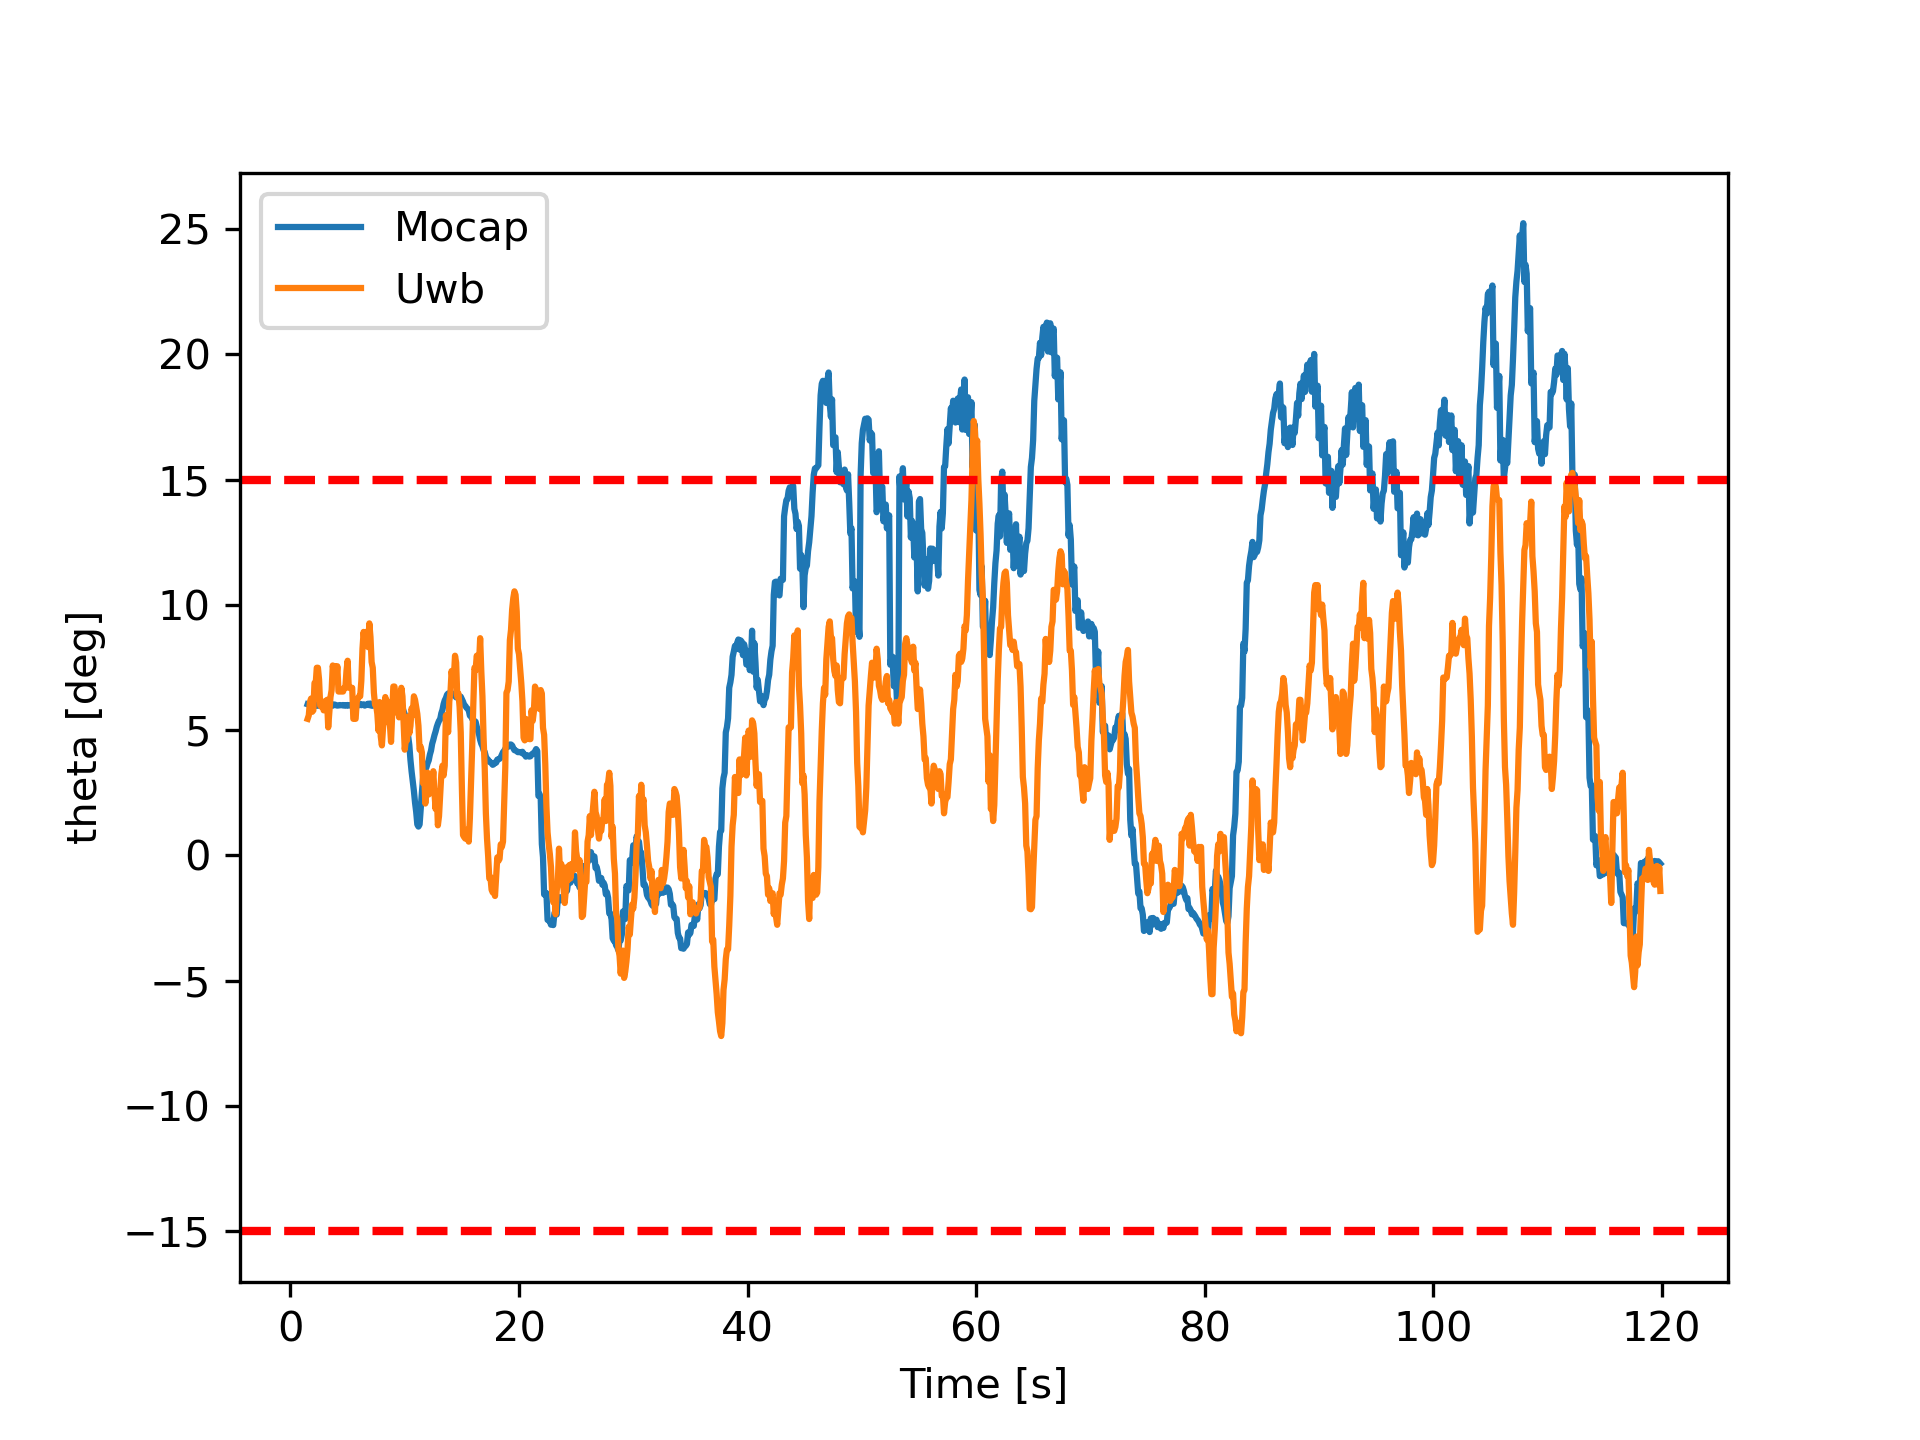
\includegraphics[width=0.48\textwidth]{images/real_test/aoa_Uwb_Mocap.png}
    \caption{angle of arrival between drone and target. The sensor measure, is compered with the one obtained with MoCap. The red dotted line, indicates the wanted range from the following policy}
    \label{REAL:fig:aoa}
\end{figure}

\begin{figure}
    \centering
    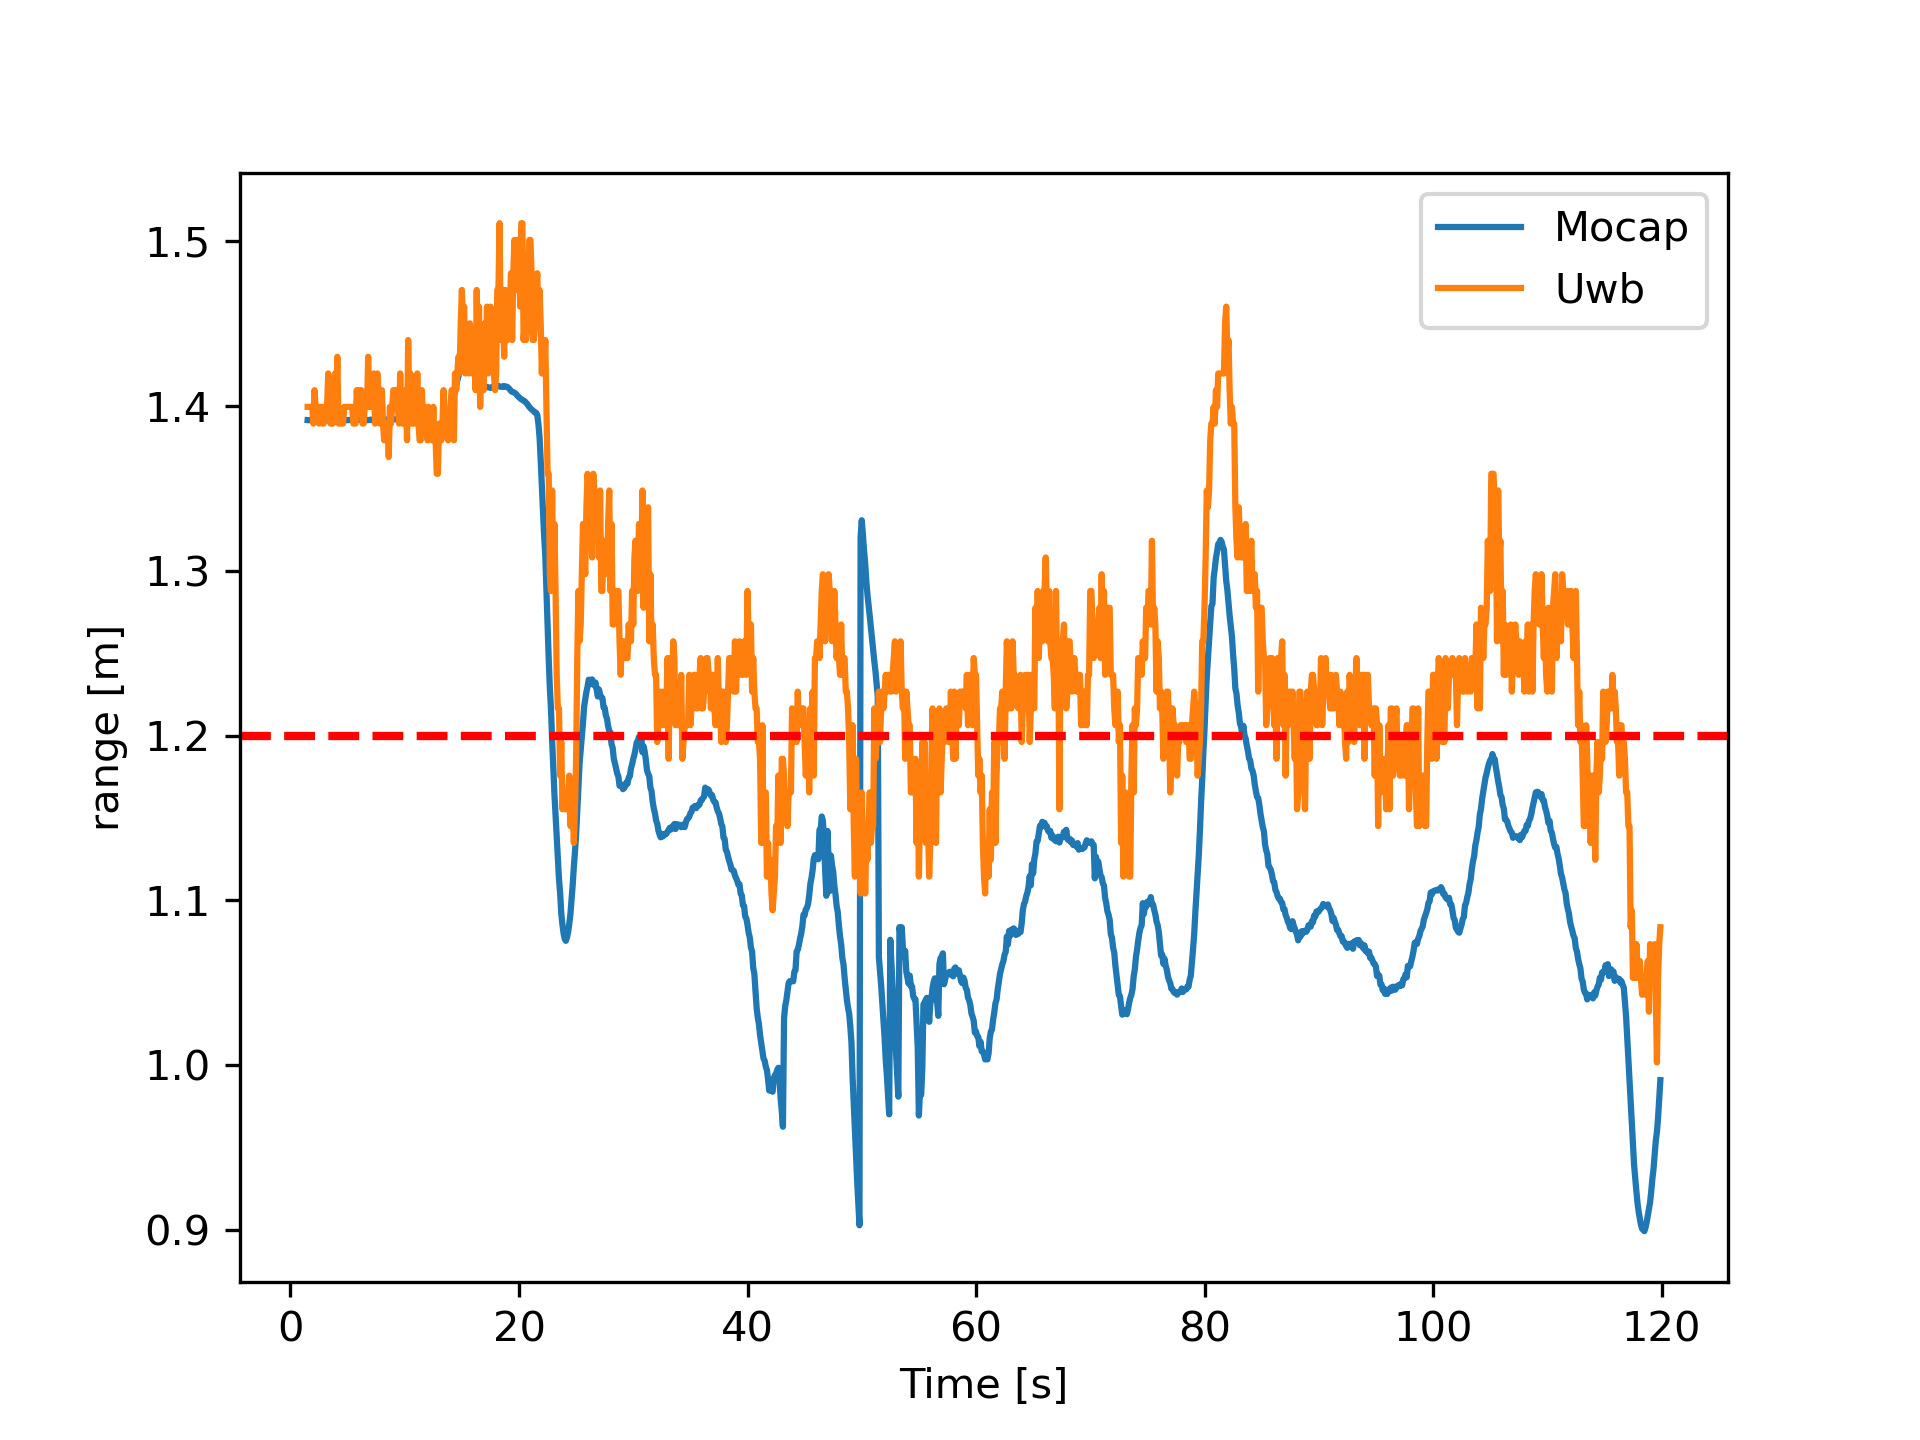
\includegraphics[width=0.48\textwidth]{images/real_test/range_Uwb_Mocap.png}
    \caption{Range between drone and target. The sensor measure, is compered with the one obtained with MoCap.}
    \label{REAL:fig:range}
\end{figure}

In conclusion this test brings up the UWB problems discussed in \autoref{UWB_CHAR}, affecting the final results. Overall the drone behaviour itself, is quite good, and the target localization remains bounded in an acceptable range. As stated, the performance could be better in larger environments with greater following distance. Further tests in this direction, are advised as future work.

\begin{figure}
    \centering
    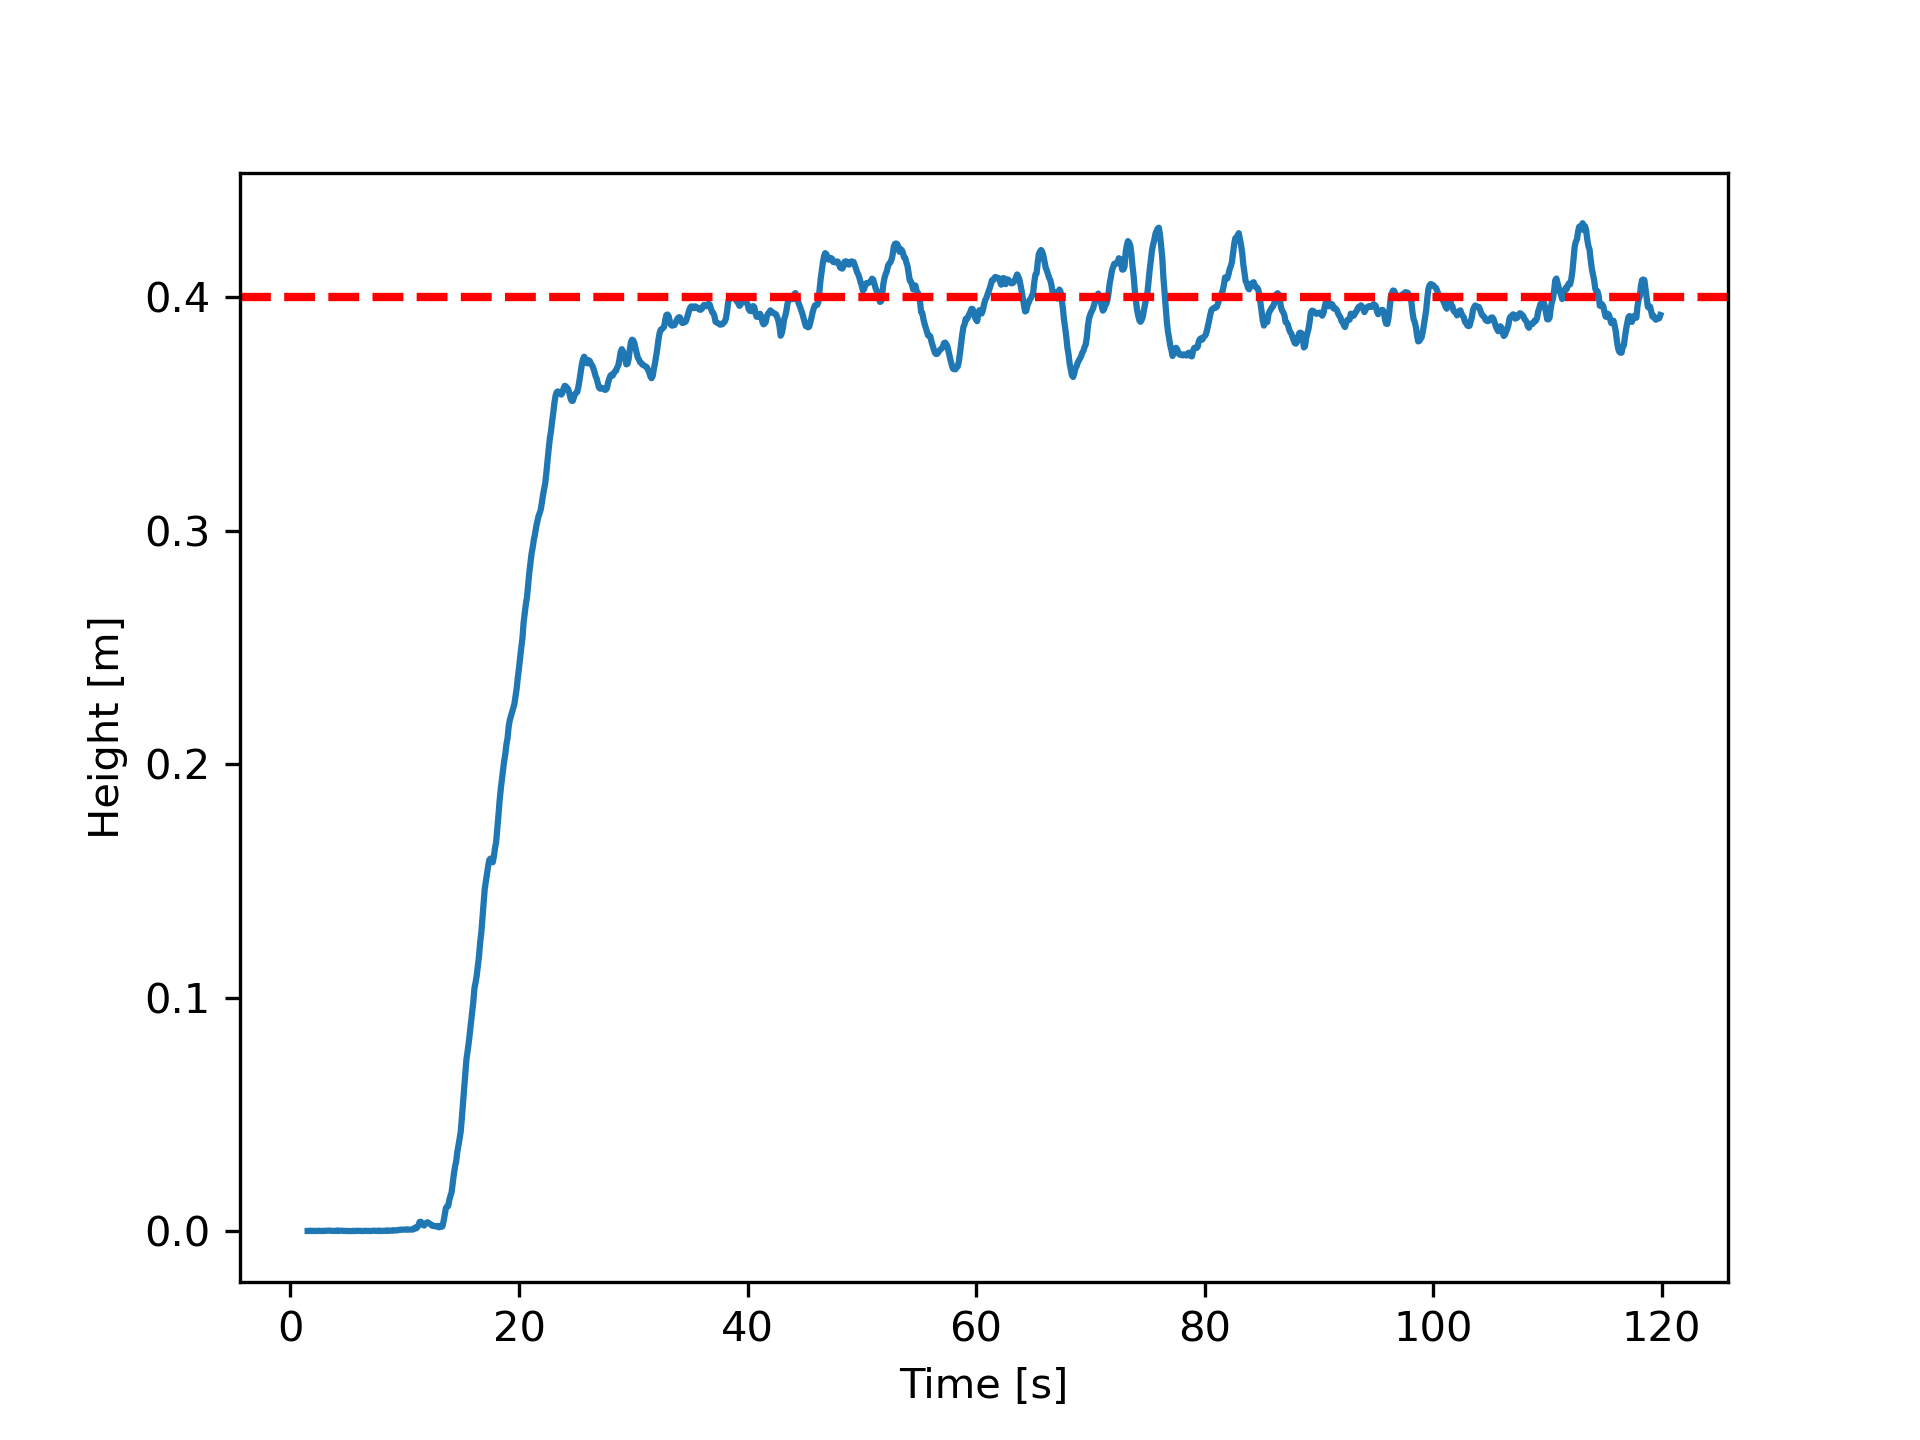
\includegraphics[width=0.48\textwidth]{images/real_test/drone_height.png}
    \caption{Measured flight height. The red dotted line, indicates the wanted height from the following policy.}
    \label{REAL:fig:height}
\end{figure}

\begin{figure}
    \centering
    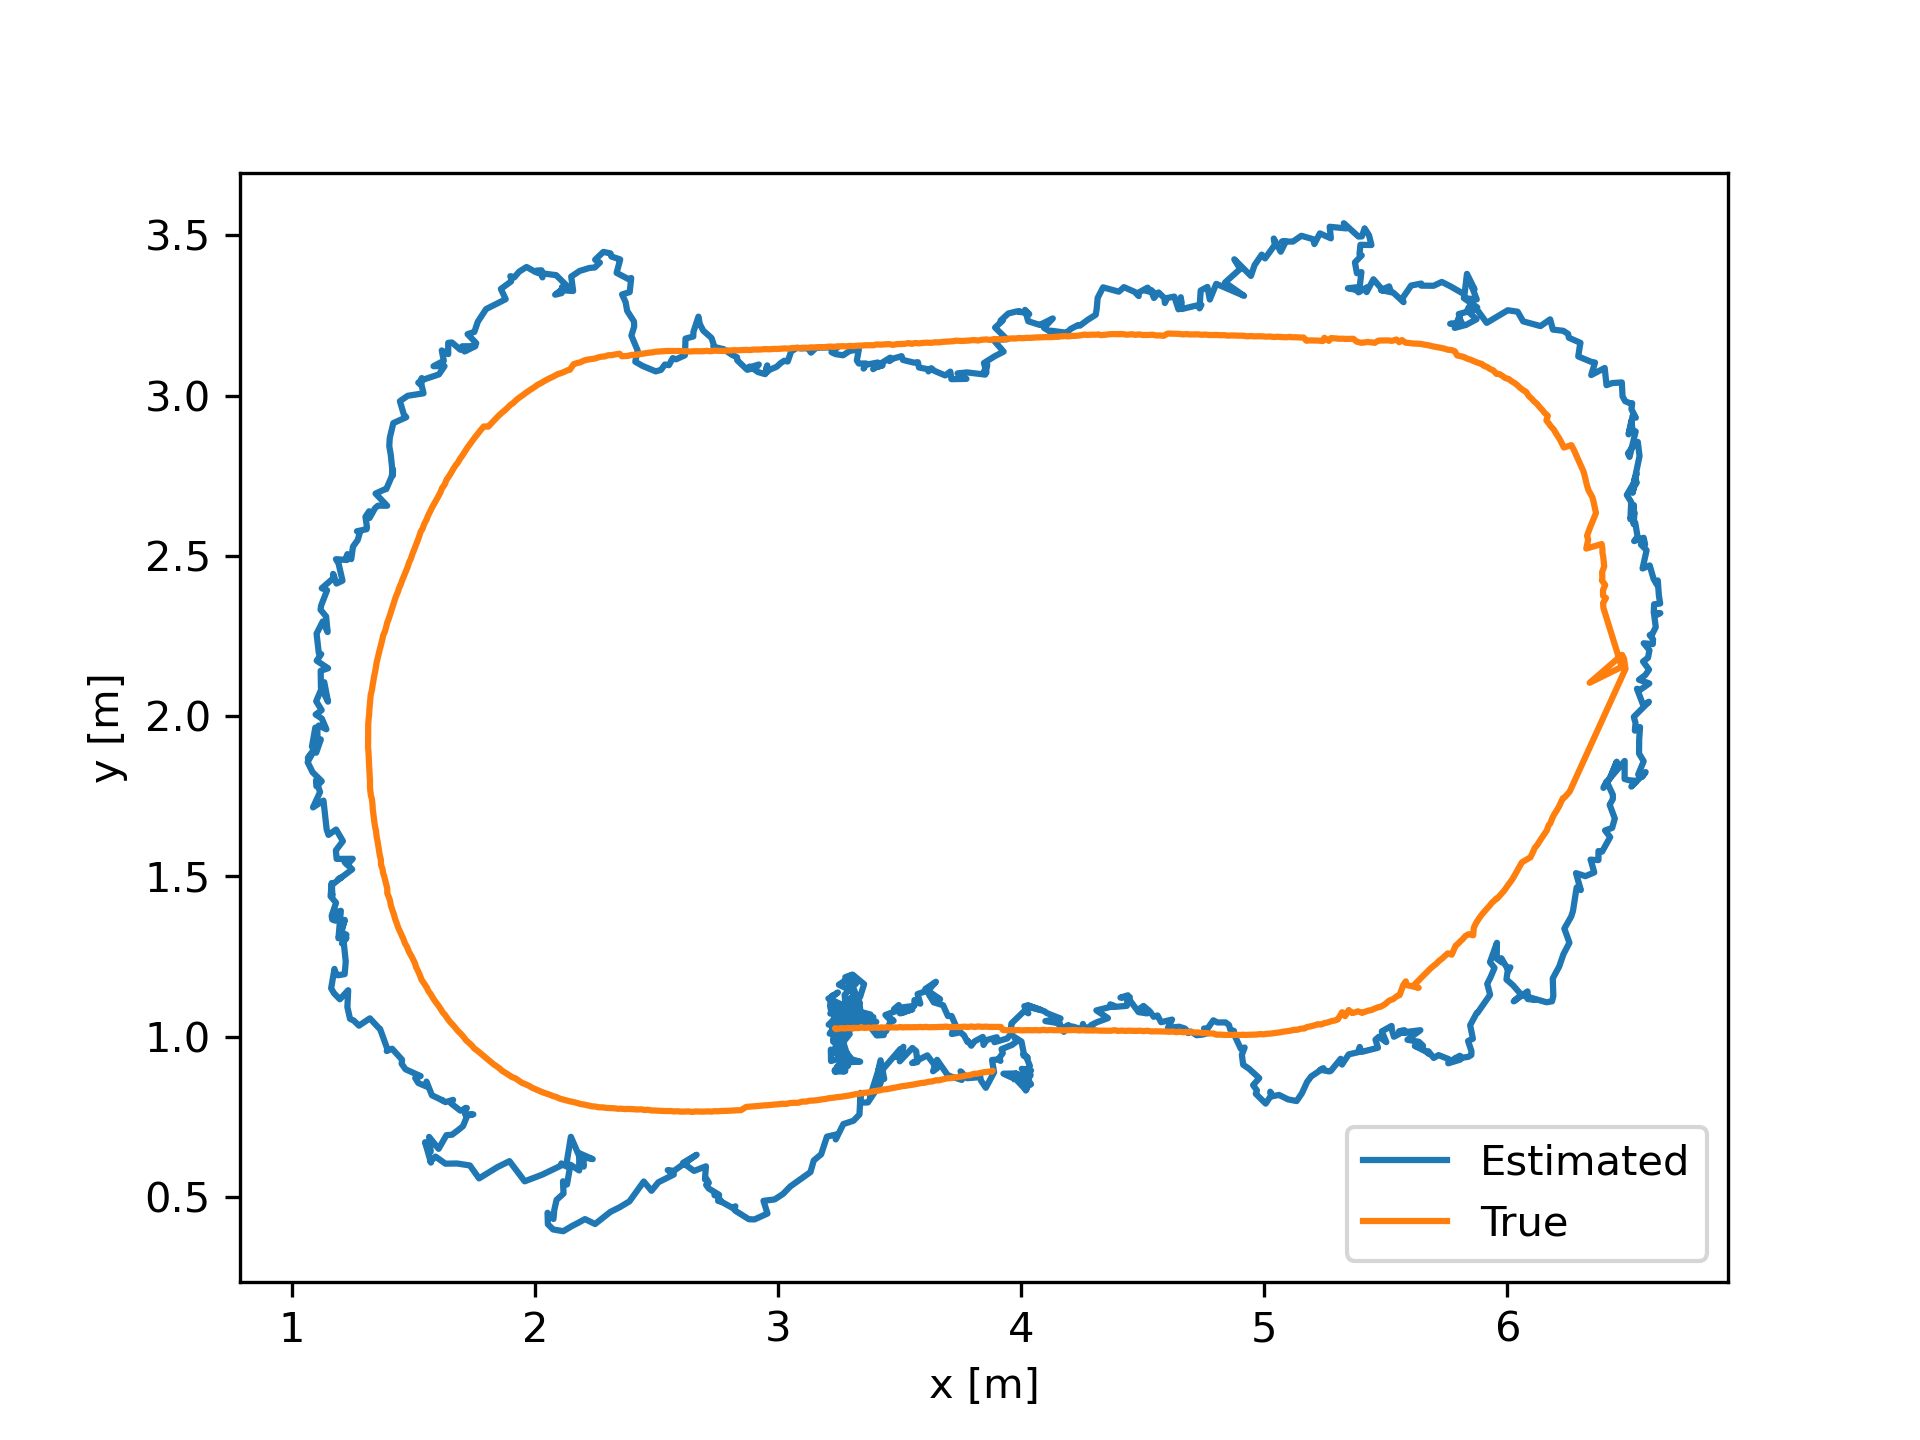
\includegraphics[width=0.48\textwidth]{images/real_test/tag_estim-real_pos.png}
    \caption{True and estimated pose of the target.}
    \label{REAL:fig:tag_estim}
\end{figure}

\begin{figure}[ht]
     \centering     
     \subfigure[]{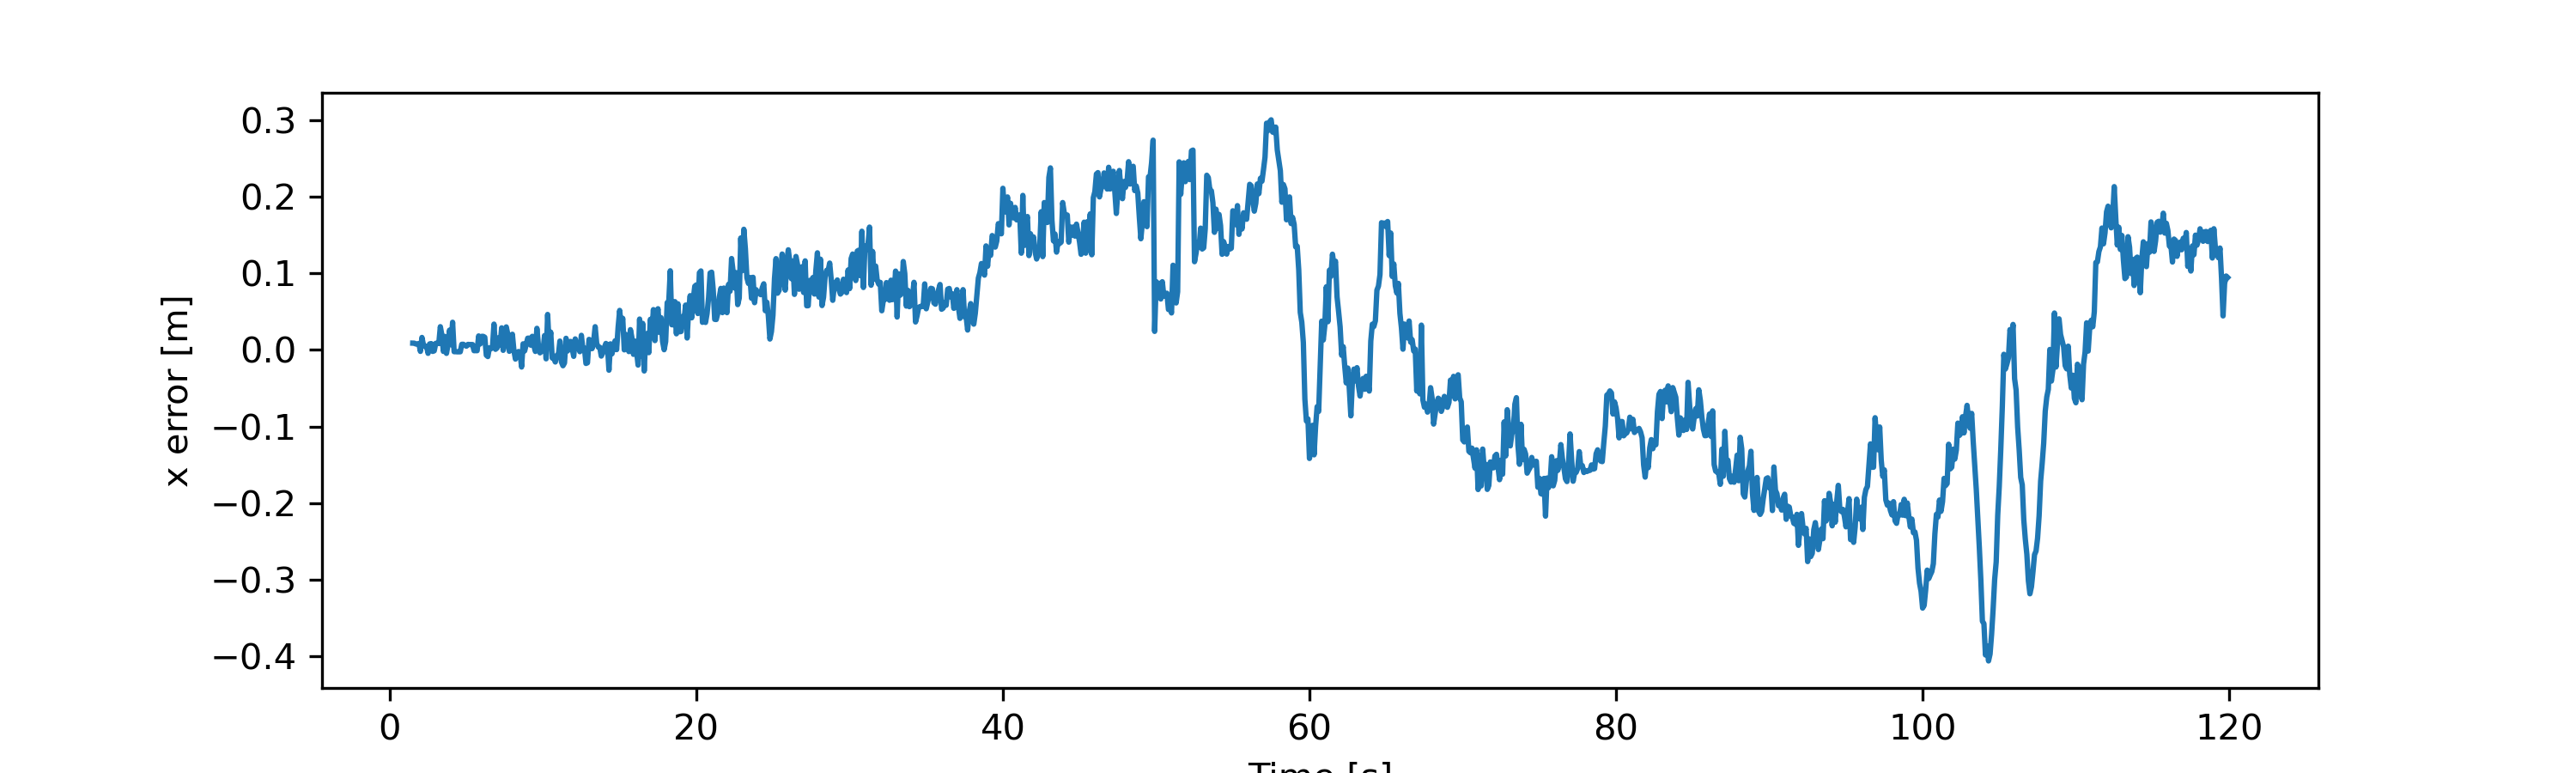
\includegraphics[width=0.48\textwidth]{images/real_test/real_tag_estimation_errx.png}}\\
     \subfigure[]{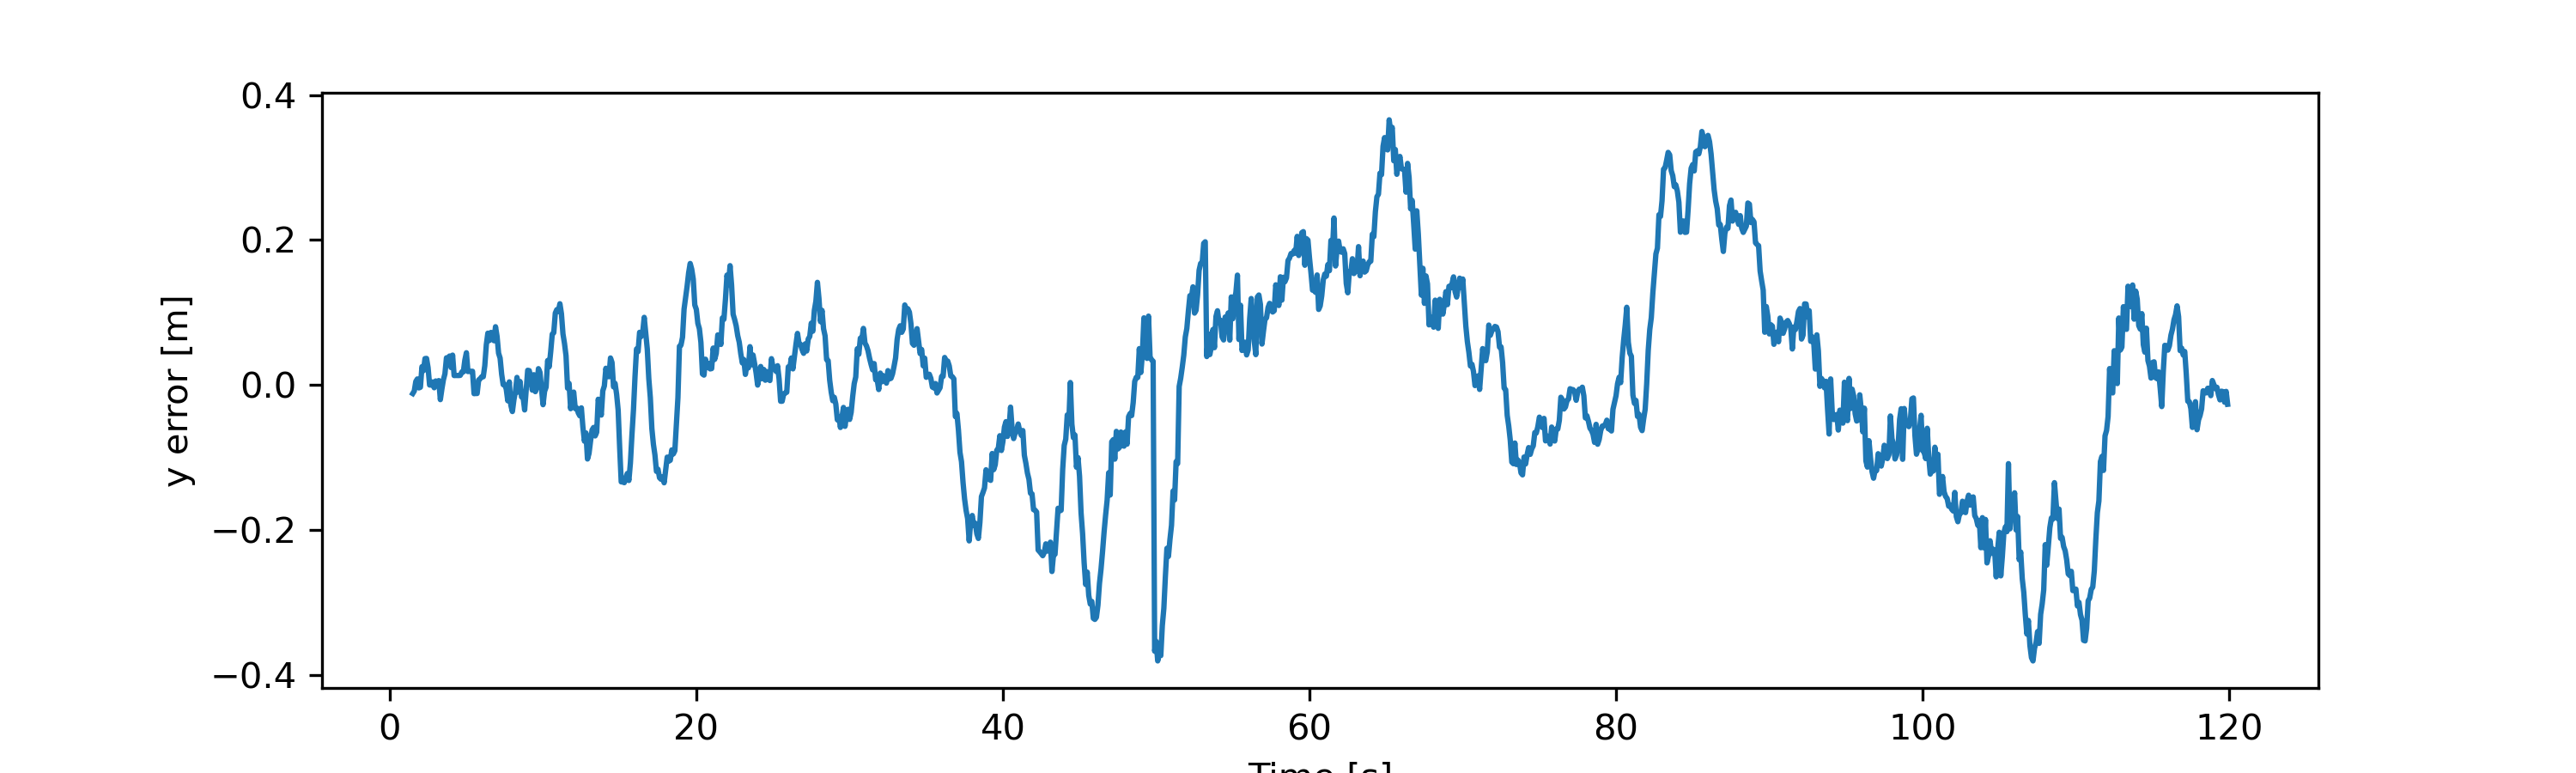
\includegraphics[width=0.48\textwidth]{images/real_test/real_tag_estimation_erry.png}}
     \caption{(a) target localization x error [m]. (b) target localization y error [m].}
     \label{REAL:fig:loc_err}
\end{figure}